\documentclass[12pt, landscape]{article}
\usepackage[scaled=0.92]{helvet}
\usepackage{multicol}
\usepackage{calc}
\usepackage{ifthen}
\usepackage[landscape]{geometry}
%\usepackage{hyperref}

\usepackage{newtxtext} 

%for strikeout
\usepackage{ulem}

%For editing parbox
\usepackage[table]{xcolor}
%For editing itemise margins, reduce iterm separaion and list separation
\usepackage{enumitem}
% For math
\usepackage{amsmath,amsthm,amsfonts,amssymb}

%For pictures / figures
\usepackage{color,graphicx,overpic}
\graphicspath{ {./../images/} }

%\usepackage{newtxtext} 
%\usepackage{amssymb}
%\usepackage[table]{xcolor}
%\usepackage{vwcol}
%\usepackage{tikz}
%\usepackage{wrapfig}
%\usepackage{makecell}


% For Code Blocks
\usepackage{xcolor}
\usepackage{listings}

% C++ Code Blocks:
\definecolor{listinggray}{gray}{0.9}
\definecolor{lbcolor}{rgb}{0.9,0.9,0.9}
\definecolor{Darkgreen}{rgb}{0,0.4,0}
\lstset{
    backgroundcolor=\color{lbcolor},
    tabsize=4,    
%   rulecolor=,
    language=[GNU]C++,
        basicstyle=\tiny,
        upquote=true,
        aboveskip={0.5\baselineskip},
	% Represents top margin
        columns=fixed,
        showstringspaces=false,
        extendedchars=false,
        breaklines=true,
        prebreak = \raisebox{0ex}[0ex][0ex]{\ensuremath{\hookleftarrow}},
        frame=single,
	% Remove Numbers
        numbers=none,
        showtabs=false,
        showspaces=false,
        showstringspaces=false,
        identifierstyle=\ttfamily,
        keywordstyle=\color[rgb]{0,0,1},
        commentstyle=\color[rgb]{0.026,0.112,0.095},
        stringstyle=\color[rgb]{0.627,0.126,0.941},
        % numberstyle=\color[rgb]{0.205, 0.142, 0.73},
%        \lstdefinestyle{C++}{language=C++,style=numbers}’.
}
\lstset{
    backgroundcolor=\color{lbcolor},
    tabsize=4,
  language=C++,
  captionpos=b,
  tabsize=3,
  frame=lines,
  % Remove Numbers
  numbers=none,
  numberstyle=\tiny,
  numbersep=3 pt,
  breaklines=true,
  showstringspaces=false,
  basicstyle=\tiny,
%  identifierstyle=\color{magenta},
  keywordstyle=\color[rgb]{0,0,1},
  commentstyle=\color{Darkgreen},
  stringstyle=\color{red}
}
% \lstset{language=C++}
%% Different languages: SQL, C++, Python


%Helpful:
%[linewidth = 1.0 \linewidth]
%\lstinline{}
% use \code{} for \lstinline with colorbox.
\newcommand{\code}[1]{\colorbox{gray!25!}{\lstinline[basicstyle=\scriptsize]|#1|}}

% Template: Cheatsheet with code enabled

%--------------------------- PACKAGES ABOVE --------------------------------------------------------------

\pdfinfo{
  /Title (CS2100 Summary.pdf)
  /Creator (Ger Teck)
  /Author (Ger Teck)
  /Subject ()
  /Keywords (tex)}

%% Margins for PAPER

% This sets page margins to .5 inch if using letter paper, and to 1cm
% if using A4 paper. (This probably isn't strictly necessary.)
% If using another size paper, use default 1cm margins.
\ifthenelse{\lengthtest { \paperwidth = 11in}}
	{ \geometry{top=.5in,left=.5in,right=.5in,bottom=.5in} }
	{\ifthenelse{ \lengthtest{ \paperwidth = 297mm}}
		{\geometry{top=1cm,left=1cm,right=1cm,bottom=1cm} }
		{\geometry{top=1cm,left=1cm,right=1cm,bottom=1cm} }
	}

% Turn off header and footer
\pagestyle{empty}

% for tight centres (less spacing)
\newenvironment{tightcenter}{%
  \setlength\topsep{0.5pt}
  \setlength\parskip{0.5pt}
  \begin{center}
}{%
  \end{center}
}

% Redefine section commands to use less space
\makeatletter
\renewcommand{\section}{\@startsection{section}{1}{0mm}%
                                {-1ex plus -.5ex minus -.2ex}%
                                {0.5ex plus .2ex}%x
                                {\normalfont\large\bfseries}}
\renewcommand{\subsection}{\@startsection{subsection}{2}{0mm}%
                                {-1explus -.5ex minus -.2ex}%
                                {0.5ex plus .2ex}%
                                {\normalfont\normalsize\bfseries}}
\renewcommand{\subsubsection}{\@startsection{subsubsection}{3}{0mm}%
                                {-1ex plus -.5ex minus -.2ex}%
                                {1ex plus .2ex}%
                                {\normalfont\small\bfseries}}
% change font
%\renewcommand{\familydefault}{\sfdefault}
%\renewcommand\rmdefault{\sfdefault}
\linespread{1.05}

\makeatother

% Define BibTeX command
\def\BibTeX{{\rm B\kern-.05em{\sc i\kern-.025em b}\kern-.08em
    T\kern-.1667em\lower.7ex\hbox{E}\kern-.125emX}}

% Don't print section numbers
\setcounter{secnumdepth}{0}

\setlength{\parindent}{0pt}
\setlength{\parskip}{0pt plus 0.5ex}

%% this changes all items (enumerate and itemize, reduce margins) ITEMIZE SEPARATION HERE
\setlength{\leftmargini}{0.5cm}
\setlength{\leftmarginii}{0.5cm}
\setlist[itemize,1]{leftmargin=2mm,labelindent=1mm,labelsep=1mm, itemsep = 0mm}
\setlist[itemize,2]{leftmargin=4mm,labelindent=1mm,labelsep=1mm, itemsep = 0mm}
%itemsep = 0mm
%\setlist{nosep}

% Need Logo Picture
%Watermark Top Right
%\usepackage{atbegshi,picture}
%\AtBeginShipout{\AtBeginShipoutUpperLeft{%
 % \put(\dimexpr\paperwidth-1.2cm\relax, -1.2cm){\makebox[0pt][r]{\framebox{
\includegraphics[width = 0.3cm]{mountainbooks} Ger Teck}}}%
%}}

% Justify Package
\usepackage[document]{ragged2e}

% -------------------------------------------------------------------------------

% START OF DOCUMENT HERE

\begin{document}
\raggedright
\footnotesize
\begin{multicols*}{3}



% multicol parameters
% These lengths are set only within the two main columns
%\setlength{\columnseprule}{0.25pt}
\setlength{\premulticols}{1pt}
\setlength{\postmulticols}{1pt}
\setlength{\multicolsep}{1pt}
\setlength{\columnsep}{2pt}

%% DOCUMENT NAME HERE
\begin{center}
     \Large{\textbf{CS2100 Comp Org Mids Notes}} \\
\end{center}
AY23/24 Sem 1, github.com/gerteck

\section{0. Computer Organisation}
\justify{
\begin{itemize}
\item Instruction set architecture (ISA) is the software stack and below it is the hardware stack.
\item High level programming language $\rightarrow$ Assembly Language $\rightarrow$ Machine Code
\item We first simplify the processor to three components: Arithmetic Logic Unit (ALU), Control Unit and Memory Unit.
\end{itemize}
 }

\section{1. C syntax}
\begin{lstlisting}
#include <iostream>
#include <stdio.h>
int main(void) {
  printf("Hello World!\n");
  std::cout << "Hello World!\n";
  return 0;
}
\end{lstlisting}
• C programs generally structured as such: 
\begin{lstlisting}
#preprocessor directives
main function header {
	declaration of variables
	executable statements
}
\end{lstlisting}
• \textbf{Preprocessor:} Starts with \#, \code{\#include} allows us to use codes defined in another file, \code{\#define} allows us to define a constant. \\
• Always declare variables at the beginning of a function, and initialize (assign initial value) before use. \\
• Three common C preprocessors: Header file inclusion, Macro expansions, conditional compilations.
\centerline{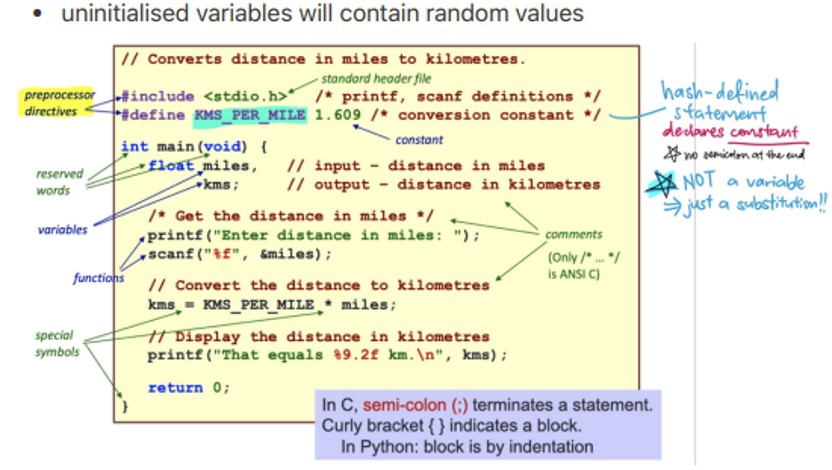
\includegraphics[width=1\linewidth]{csyntax}} 

\begin{itemize}
	\item C is \textbf{statically typed} language, type is the \textbf{property of the variable}. Once declared, variable can only store data of particular type. 
\end{itemize}
\textbf{Variable attributes: Name, Type, Address, Value}. \\
• Names are case-sensitive, camelCase, PascalCase.  \\
• All data in C is (or can be) represented as integers. Characters are represented by 8-bit "char" integers based on the ASCII table. \\
• Strings are then represented as: Array of char. Terminated by a null character (' $\backslash$0' or 0) 


\subsubsection{Primitive Data Types in C:} 
\centerline{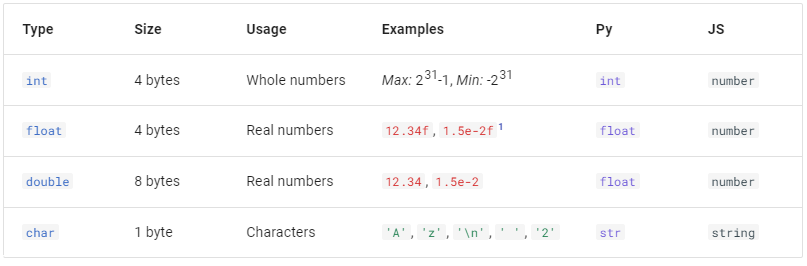
\includegraphics[width=1\linewidth]{datatypes}} 
\centerline{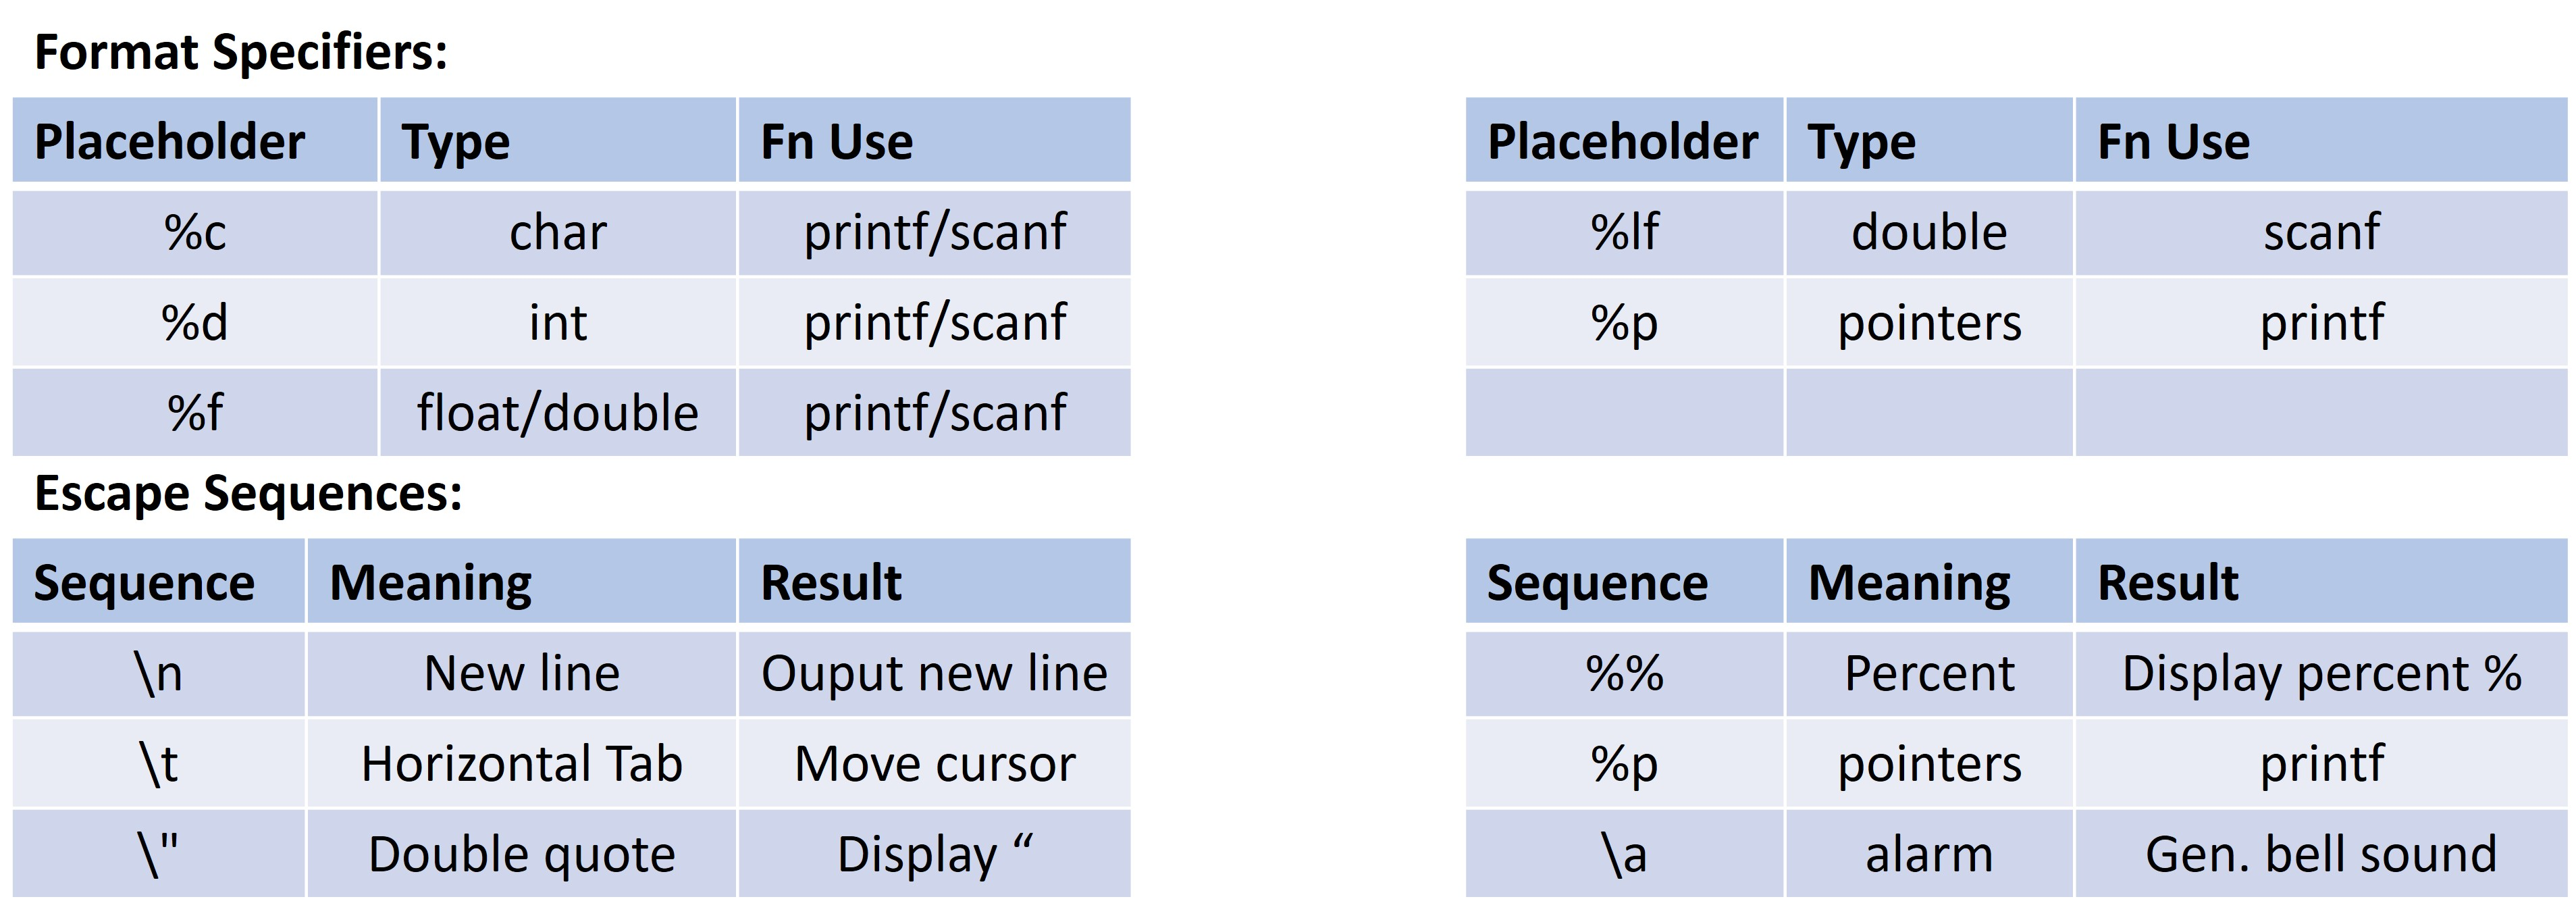
\includegraphics[width=1\linewidth]{specifiers}}
{Typecasting in C:}
\begin{lstlisting}
/* syntax: (type) expression */
int ii = 5; float ff = 15.34
float a = (float) ii / 2; // a = 2.5
float b = (float) (ii / 2); // b = 2.0, floor division
int c = (int) ff / ii; // c = 3
\end{lstlisting} 

\justify{
\subsubsection{Assignment Statements}
• The value assigned is returned as result of evaluation.
\begin{lstlisting}
a = b = c = 3 + 6;	// is possible
a = 5 + (b = 3);		// b = 3, a = 8
\end{lstlisting} }
\center{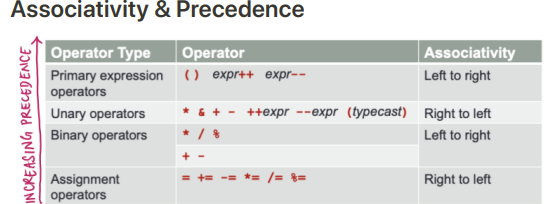
\includegraphics[width=0.95\linewidth]{associativity}}
 
\justify{
\subsubsection{Selection}
• We may define our own boolean library or (\code{#include <stdbool.h>}).  \\
Non-zero values treated as true, but only 1 (==) equal true. 
\begin{lstlisting}
#define false 0
#define true  1
#define bool  char
\end{lstlisting}
• Short-circuit evaluation.

\subsubsection{switch/case:} 
• \textbf{fall through behavior}: Removal of \code{break} allows subsequent cases to run.
\begin{lstlisting}
switch(<variable_or_expression>) {
  case value1:
    /* ... */
    break; // Prevents spill over to next case

  case value2:
    /* ... */
    // no break can spill over to next case

  case value3:
    /* ... */
    break;
  
   default: // code to execute if equal none.
    /* ... */
    break;
}
\end{lstlisting}
}
\subsubsection{loops:} 
\centerline{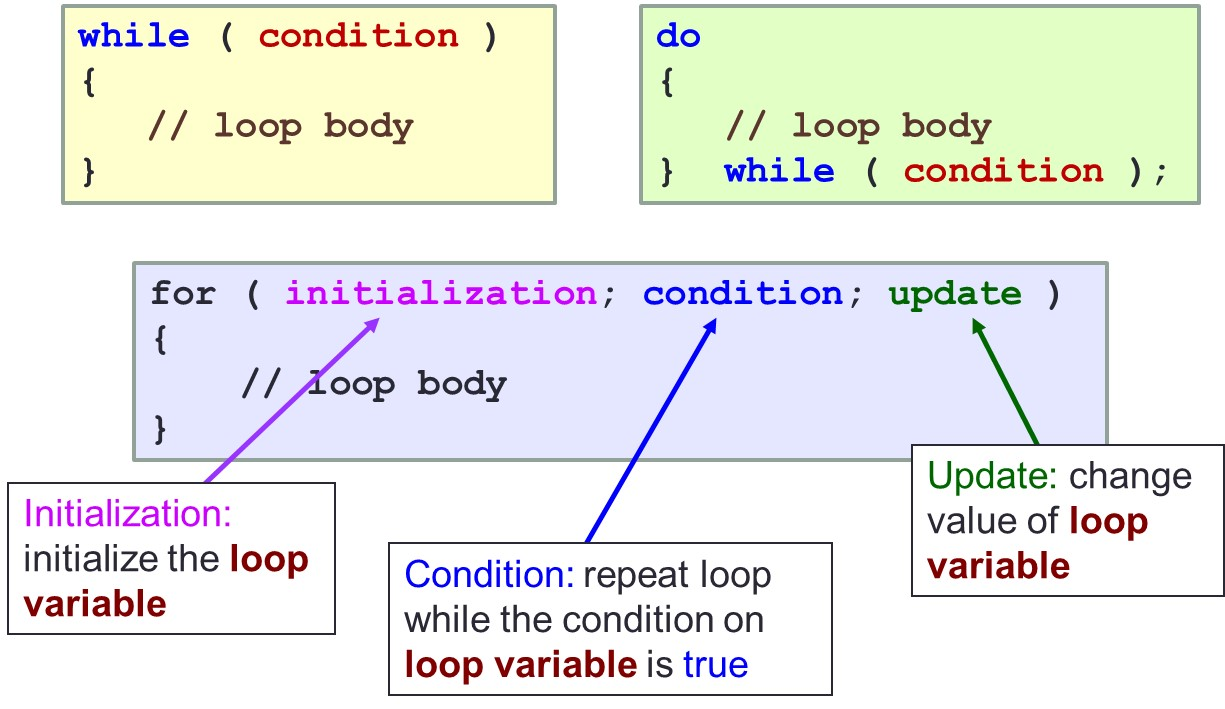
\includegraphics[width=1\linewidth]{loops}}

\vfill\null
\columnbreak


\section{2. C syntax (Pointers \& Functions)}
Every \textbf{memory location} in a computer is indexed with an address. \\
All variables in C must be stored in memory, 
\begin{lstlisting}
int main(void) {
	int a = 3, *b; 	// b is a pointer to an int
 	b = &a; 				// b points to the address of a
	*b = 5; 				// set a through b, a=5	

	int *a_ptr;
	a_ptr = &a;
}
\end{lstlisting}
\begin{itemize}
	\item \textbf{pointer variable} stores the address of another variable.
	\item \textbf{\&} $\rightarrow$ address operator. \\
\code{\&x} $\rightarrow$ address of memory cell where value of x is stored, gets address of a variable.

	\item \code{*} $\rightarrow$ declares a pointer. \\
\code{type *pointer_name} (e.g. \code{int *x} )

	\item \code{*} - dereferencing (access variable through pointer) \\
\code{ *x = 32}: following through the pointer to get the value

	\item Incrementing a pointer('s pointed value): \code{(*p)++;} \\
without brackets: increments pointer to next address (depending
on size of the data type) aka += sizeof(*p1)
	
\end{itemize}
\begin{lstlisting}
double a, *b;
b = &a; // legal
double c, d;
*d = &c; // legal
double e, f;
f = &e; // ILLEGAL!
\end{lstlisting}

\subsubsection{Call-by-Value / Pointer}
\begin{itemize}
	\item In C, the actual parameters are passed to the formal parameters by a mechanism known as call-by-value. 
	\item The only way for a function to modify the value of a variable outside its scope, is to use pointers to access that variable. (Call-by-pointer)

\end{itemize}

\vfill\null
\columnbreak

\section{3. C Arrays, Strings \& Structs}
\textbf{Arrays}
\begin{itemize}
	\item a homogenous collection of data all of the same type, occupying contiguous memory locations.
	\item  declaration: \code{arr = elementType[size]}
	\item arr refers to \code{\&arr[0]}
	\item an array name is a \textbf{fixed (constant) pointer}, which points to the first element in the array and cannot be reassigned - \code{arr1 = arr2} is illegal.
\end{itemize}
\begin{lstlisting}
// an array can ONLY be initialised at the time of declaration.
int evens[5] = {2, 4, 6, 8, 10};
// if you initialise values, no need to declare length
int odds[] = {1, 3, 5};
// uninitialised values will be zero value
int some[5] = {1, 2, 3}; // some = [1, 2, 3, 0, 0]

int numbers[3];
printf("Enter 3 integers:");
for (i = 0; i < 3; i++) {
 scanf("%d", &numbers[i]); }
\end{lstlisting}

\textbf{In function prototypes}
\begin{lstlisting}
// parameter names are optional
int sumArray(int [], int); // valid
int sumArray(int arr[], int size); // valid
int sumArray(int *, int); // pointer is valid too

// size can be specified but will be ignored
int sumArray(int arr[8], int size); 

// function definition
int sumArray(int *arr, int size) { ... }
int sumArray(int arr[8], int size) { ... } // size ignored
\end{lstlisting}

\textbf{Strings}
\begin{itemize}
\item array of characters terminated with a null character: $\backslash$ 0, which has ASCII value of 0.
\item string functions: \code{\#include <string.h>}
\end{itemize}

\begin{lstlisting}
char my_str[] = "hello";
char my_str[] = {'h', 'e', 'l', 'l', 'o', '\0'};
\end{lstlisting}

\subsubsection{I/O}
\begin{itemize}
	\item \code{in}: \code{fgets(str, size, stdin)} reads (size - 1) chars or until newline encountered.
	\item \code{in}: \code{scanf("\%s", str)} - reads until whitespace.
	
	\item \code{out}: \code{puts(str)} - terminates with newline
	\item \code{out}: \code{printf("\%s\n", str)} - prints until '$\backslash$0' in \code{str} encountered.
\end{itemize}

\subsubsection{String functions}
\begin{itemize}
	\item \code{strlen(s)}: returns number of characters in s up to '$\backslash$0'
	\item \code{strcmp(s1, s2)}: compares the ASCII values of corresponding characters, returns s1 - s2, negative number / positive number / 0 if they are equal.
	\item \code{strncmp(s1, s2, n)}: strcmp for first n characters of s1 and s2
	\item \code{strcpy(s1, s2)}: copy s2 into s1, ◦cannot directly assign s1 = "Hello", but can copy: strcpy(s1, "Hello")
	\item \code{strncpy(s1, s2, n)}: copy first n characters of s2 into s1
\end{itemize}

\subsubsection{Structs}
\begin{itemize}
	\item allow grouping of heterogenous data
	\item passed by value into functions \\
unless: passing array of structs to a function \\
array members of structs are \textbf{deeply copied}
	\item can be reassigned
	\item no memory is allocated to a type.
\end{itemize}

create new types called box\_t and nested\_box\_t:
\begin{lstlisting}
// declare BEFORE function prototypes
typedef struct {
 int length, width;
 float height;
} box_t;

typedef struct {
 int id;
 box_t smaller_box;
} nested_box_t;

// initialising struct variables
box_t mybox = {2, 3, 5.1};
nested_box_t big_box = {0, {4, 3, 6.7}};

// accessing members
box.length = 1;
big_box.smaller_box.width = 2;
\end{lstlisting}

\textbf{Arrow Operator \code{->}}
\begin{itemize}
\item \code{(*player_ptr).name} is equivalent to \code{player_ptr->name}
\item \code{*player_ptr.name} means \code{*(player_ptr.name)} (dot has higher
precedence
\end{itemize}


\vfill\null
\columnbreak


\section{4. Number Systems}
\subsubsection{Data Representation}
\begin{itemize}
\item 1 byte = 8 bits
\item word = multiple of a byte (e.g. 1 byte, 2 bytes, 4 bytes) \\
64-bit machine $\rightarrow$ 1 word is 8 bytes
\item N bits can represent up $2^N$ to values
\item to represent values: ceil [$log_2M$] bits required
\end{itemize}

\subsubsection{Weighted Number systems}
\begin{itemize}
\item weighted number system $\rightarrow$ has a base (radix) \\
base/radix $R$ has weights in powers of $R$
\end{itemize}

\textbf{Prefixes in C}
\begin{itemize}
\item prefix \code{0} for octal (e.g. \code{032} = $(32)_8$ )
\item prefix \code{0x} for hexadecimal (e.g. \code{0x32} = $(32)_16$ )
\item prefix \code{0b} for binary
\end{itemize}

\subsubsection{Conversion}
\begin{itemize}
\item \textbf{decimal to binary:} \\
whole numbers: repeated \textbf{division} by 2, LSB → MSB \\
fractions: repeated \textbf{multiplication} by 2, MSB → LSB 
\item \textbf{decimal to base-R:} \\
for whole numbers: repeated \textbf{division} by R
for fractions: repeated \textbf{multiplication} by R
\item binary $\rightarrow$ octal: partition in groups of 3
\item octal $\rightarrow$ binary: convert each digit into 3-bit binary
\item binary $\rightarrow$  hexadecimal: partition in groups of 4
\item hexadecimal $\rightarrow$ binary: convert each digit to 4-bit binary
\end{itemize}

\subsubsection{ASCII}
\begin{itemize}
\item American Standard Code for Information Interchange
\item 7 bits plus 1 parity bit (for error checking): $2^7$ $= 128$
\item in C: \code{char} datatype is 1 byte = 8 bit integer \\
corresponds to ASCII - can typecast int/char \\
e.g. convert uppercase char to lowercase: \code{c = c + 'a' – 'A'}
\end{itemize}

\subsubsection{Negative Numbers}
\begin{itemize}
\item \textbf{unsigned} numbers: only non-negative values
\item \textbf{signed} numbers: include all values (positive and negative)
\item {for negating non-whole numbers:} same as whole numbers (ignore
the decimal point, then put it back)
\end{itemize}

\subsubsection{Overflow}
\begin{itemize}
\item positive + positive = negative, OR
\item negative + negative = positive
\end{itemize}
\textbf{1s addition:} If carry out, add 1 to the result (wrap around) \\
\centerline{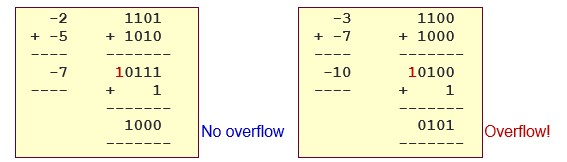
\includegraphics[width=0.9\linewidth]{1saddition}} \\
\textbf{2s addition:}: Ignore the carry out.

\subsubsection{Sign-and-Magnitude:}
\begin{itemize}
\item MSB represents the sign (0 is positive)
\item \textbf{range (8-bit):} $-127_{10}$ to $+127_{10}$ \\
2 zeroes: \code{00000000}($+0_{10}$) and \code{10000000} ($-0_{10}$)
\item \textbf{negating a number}: reverse the first bit
\item \textbf{issues} \\
1. there are two zeroes (which may be useful for limits!) \\
2. not good for performing arithmetic due to the zero in front
\end{itemize}


\subsubsection{1s Complement:}
\begin{itemize}
\item negated value of x, $-x = 2^n - x - 1$
\item \textbf{negating a number}: invert the bits
\item \textbf{range (8-bit)}: $-127_{10} $ to $+127_{10}$ \\
2 zeroes: \code{00000000} ($+0_{10}$) and \code{11111111} ($-0_{10}$ ) \\
\textbf{range (n-bits):} $-2^{n-1}$ to $2^{n-1}$
\end{itemize}

\subsubsection{2s Complement}
\begin{itemize}
\item = 1s complement + 1
\item negated value of x, $-x = 2^n - x$
\item \textbf{negating a number} \\
invert the bits, then \textbf{add 1}
\item \textbf{range (8-bit):} $-128_{10}$ to $127_10$ \\
zero: \code{00000000} = $+0_{10}$
\textbf{range (n-bits):} $-2^{n-1}$ to $2^{n-1} - 1$
\end{itemize}


\subsubsection{Excess Representation}
\begin{itemize}
\item Allows the range of values to be distributed evenly between the positive and negative values, by a simple translation.
\item \code{00..00} = $-2^n$
\item \code{10..00} = $0$
\item to express $n$ in Excess-$M$ representation: $n + M$ \\
E.g. express 5 in excess 8 (4 bit): $5 + 8 = 13$ OR \code{1101}
\end{itemize}

\section{5. Number Representations}
\subsubsection{Fixed-point representation}
\begin{itemize}
\item In fixed-point representation, the number of bits allocated for the whole number part and fractional part are fixed.
\item Issue: limited range.
\end{itemize}
\centerline{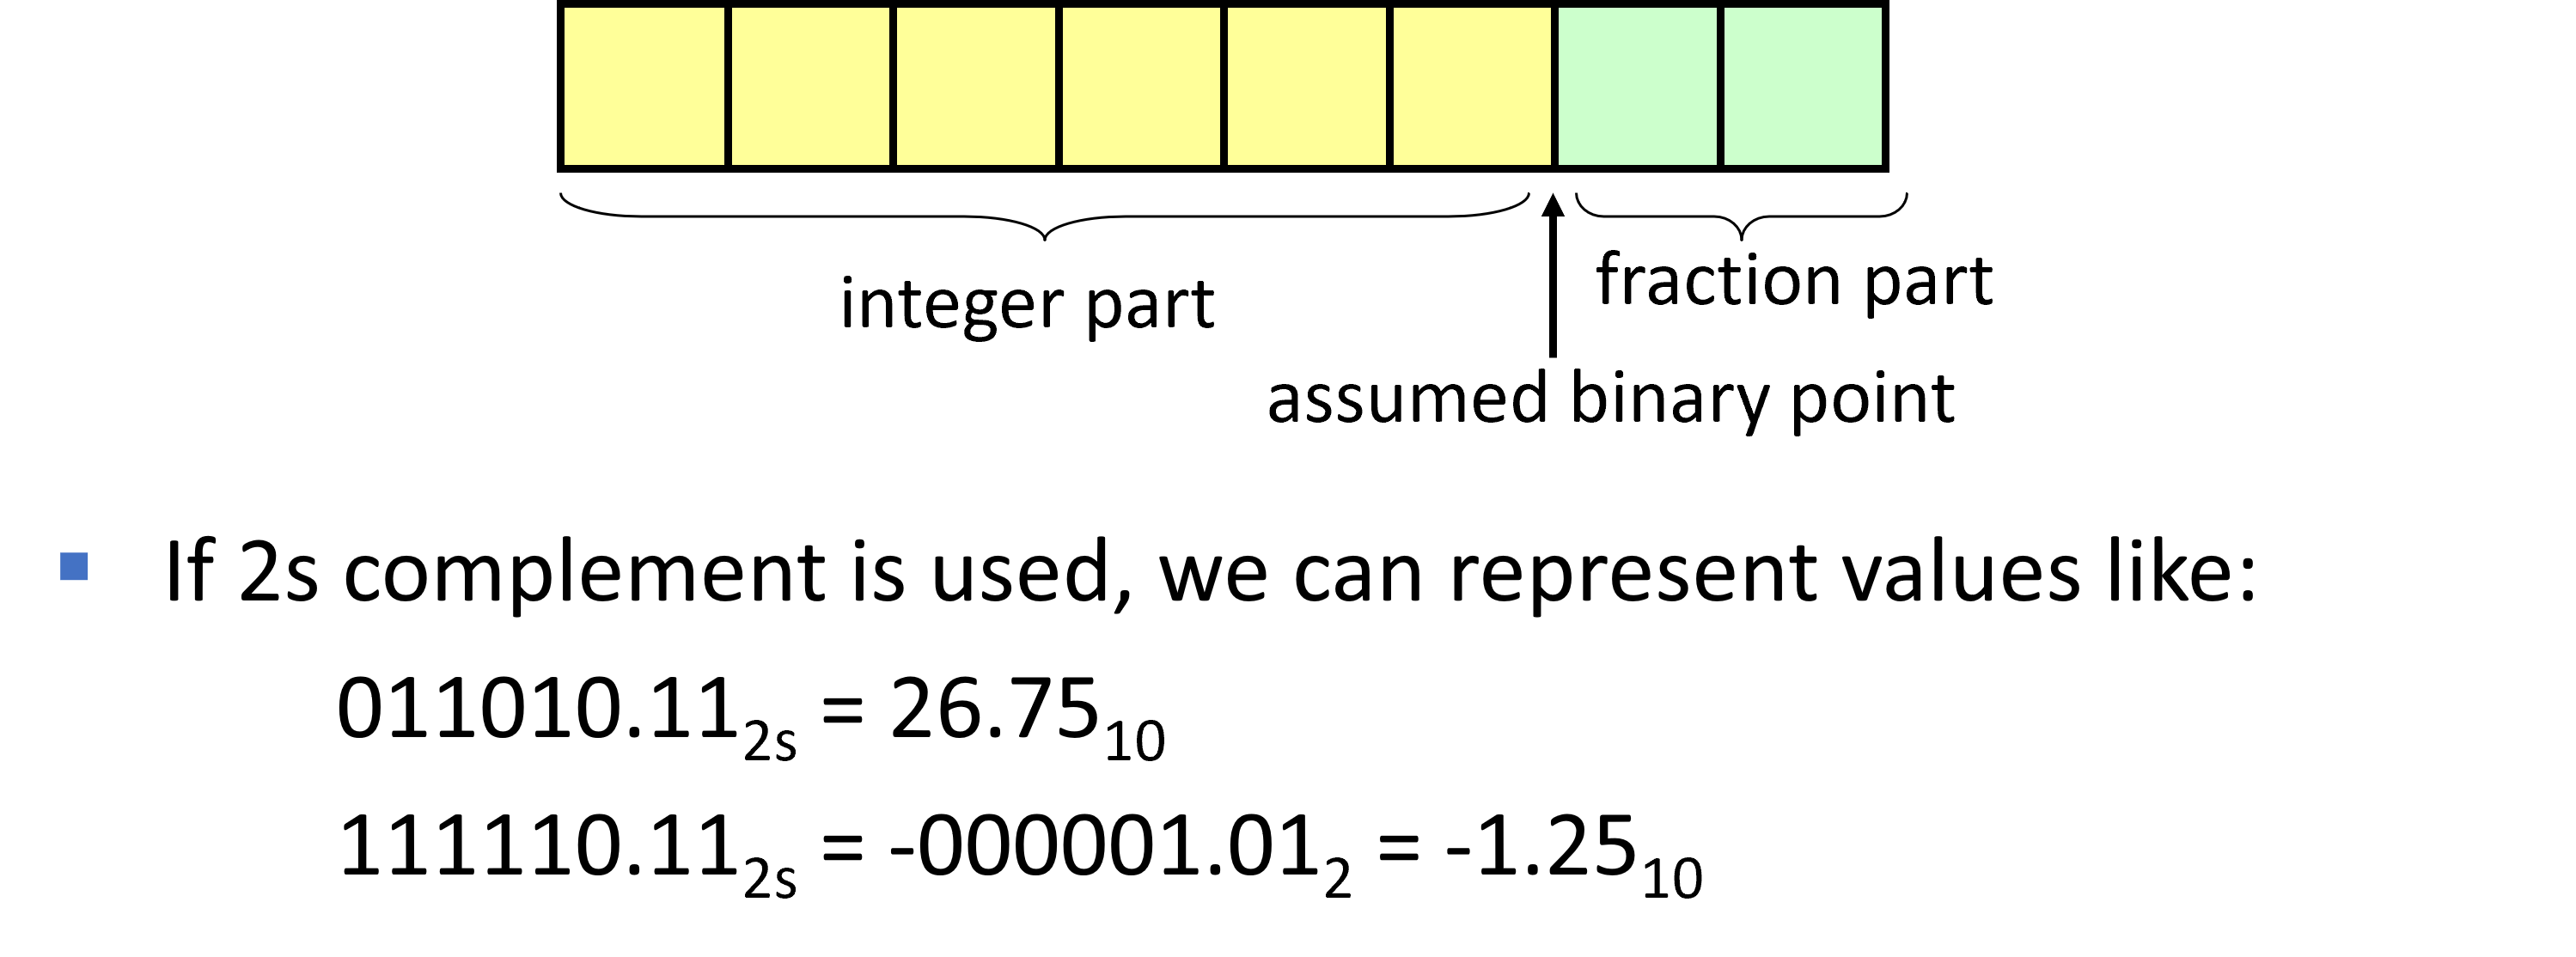
\includegraphics[width=1\linewidth]{fixedpoint}}

\subsubsection{Floating-point representation}
\begin{itemize}
\item IEEE 754 floating-point representation \\ 
◦ exponent is \textbf{excess-127}
\end{itemize}
\centerline{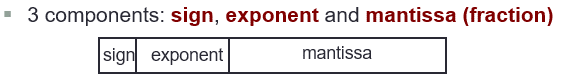
\includegraphics[width=1\linewidth]{floatpoint}}
single-precision (32 bit format): 1-bit sign / 8-bit exponent / 23-bit mantissa
\begin{itemize}
\item \textbf{mantissa} is normalised with an implicit leading bit 1 \\
to maximise the numbers to be stored \\
normalise it to  the rightmost bit is always 1, no need to store it.
\item better range and accuracy, but more complex
\end{itemize}
\centerline{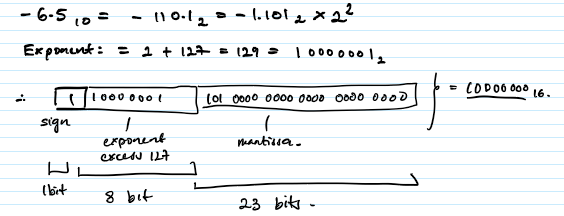
\includegraphics[width=0.8\linewidth]{IEEEexample}}



\section{6. MIPS + ISA}
\subsubsection{Instruction Set Architecture}
\begin{itemize}
\item \textbf{ISA:} abstraction of the interface between the hardware and low-level
software \\
Software is translated into the instruction set. \\
Hardware implements the instruction set.
\item \textbf{Complier} turns high level language into assembly code. \\
\textbf{Assembler} translates assembly language to machine code.
\item \textbf{stored-memory concept (von Neumann architecture)}: both instructions and data are stored in
memory.
\item \textbf{The load-store model:} *Limit memory operations and relies on registers for storage during execution.
\end{itemize}
\centerline{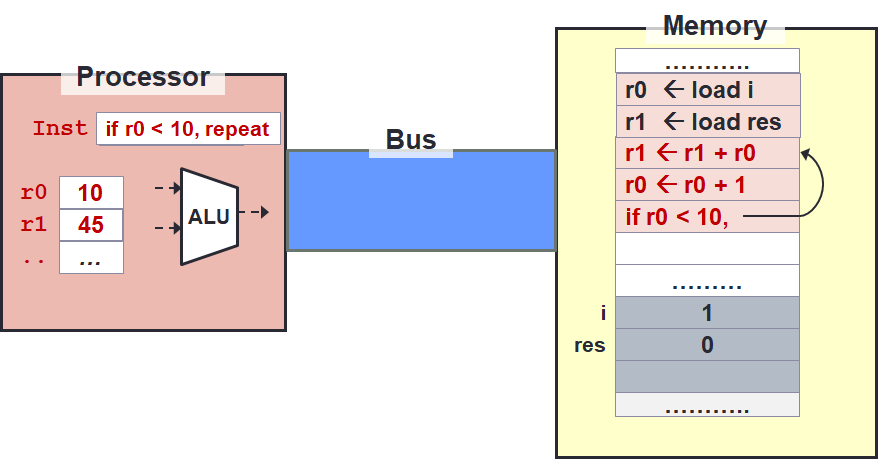
\includegraphics[width=0.8\linewidth]{isa1}}
\begin{itemize}
\item major types of assembly instruction: \\
◦ \textbf{memory}: move values between memory and registers
◦ \textbf{calculation}: arithmetic and other operations \\
◦ \textbf{control flow}: change the sequential execution (sequence in which
instructions are executed)
\end{itemize}

\subsubsection{Registers}
\begin{itemize}
\item Registers close to processors, fast speed of access. Values in registers are simply binaries, no data types associated.
\item Typical architecture has 16 to 32 registers
\item MIPS register can hold any 32-bit number
\end{itemize}
\centerline{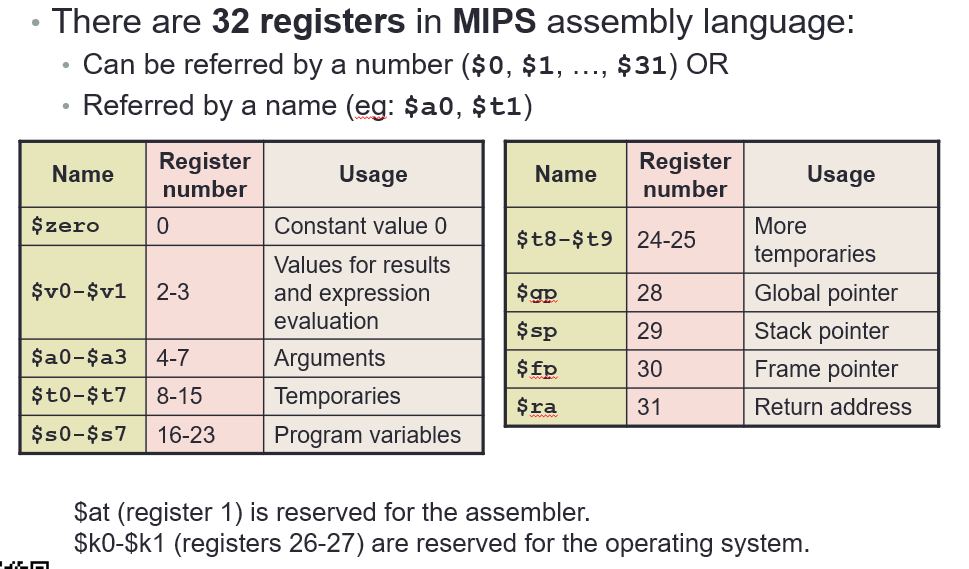
\includegraphics[width=0.8\linewidth]{registers}}

\section{6. MIPS Assembly Language}
\subsubsection{Instructions}
\centerline{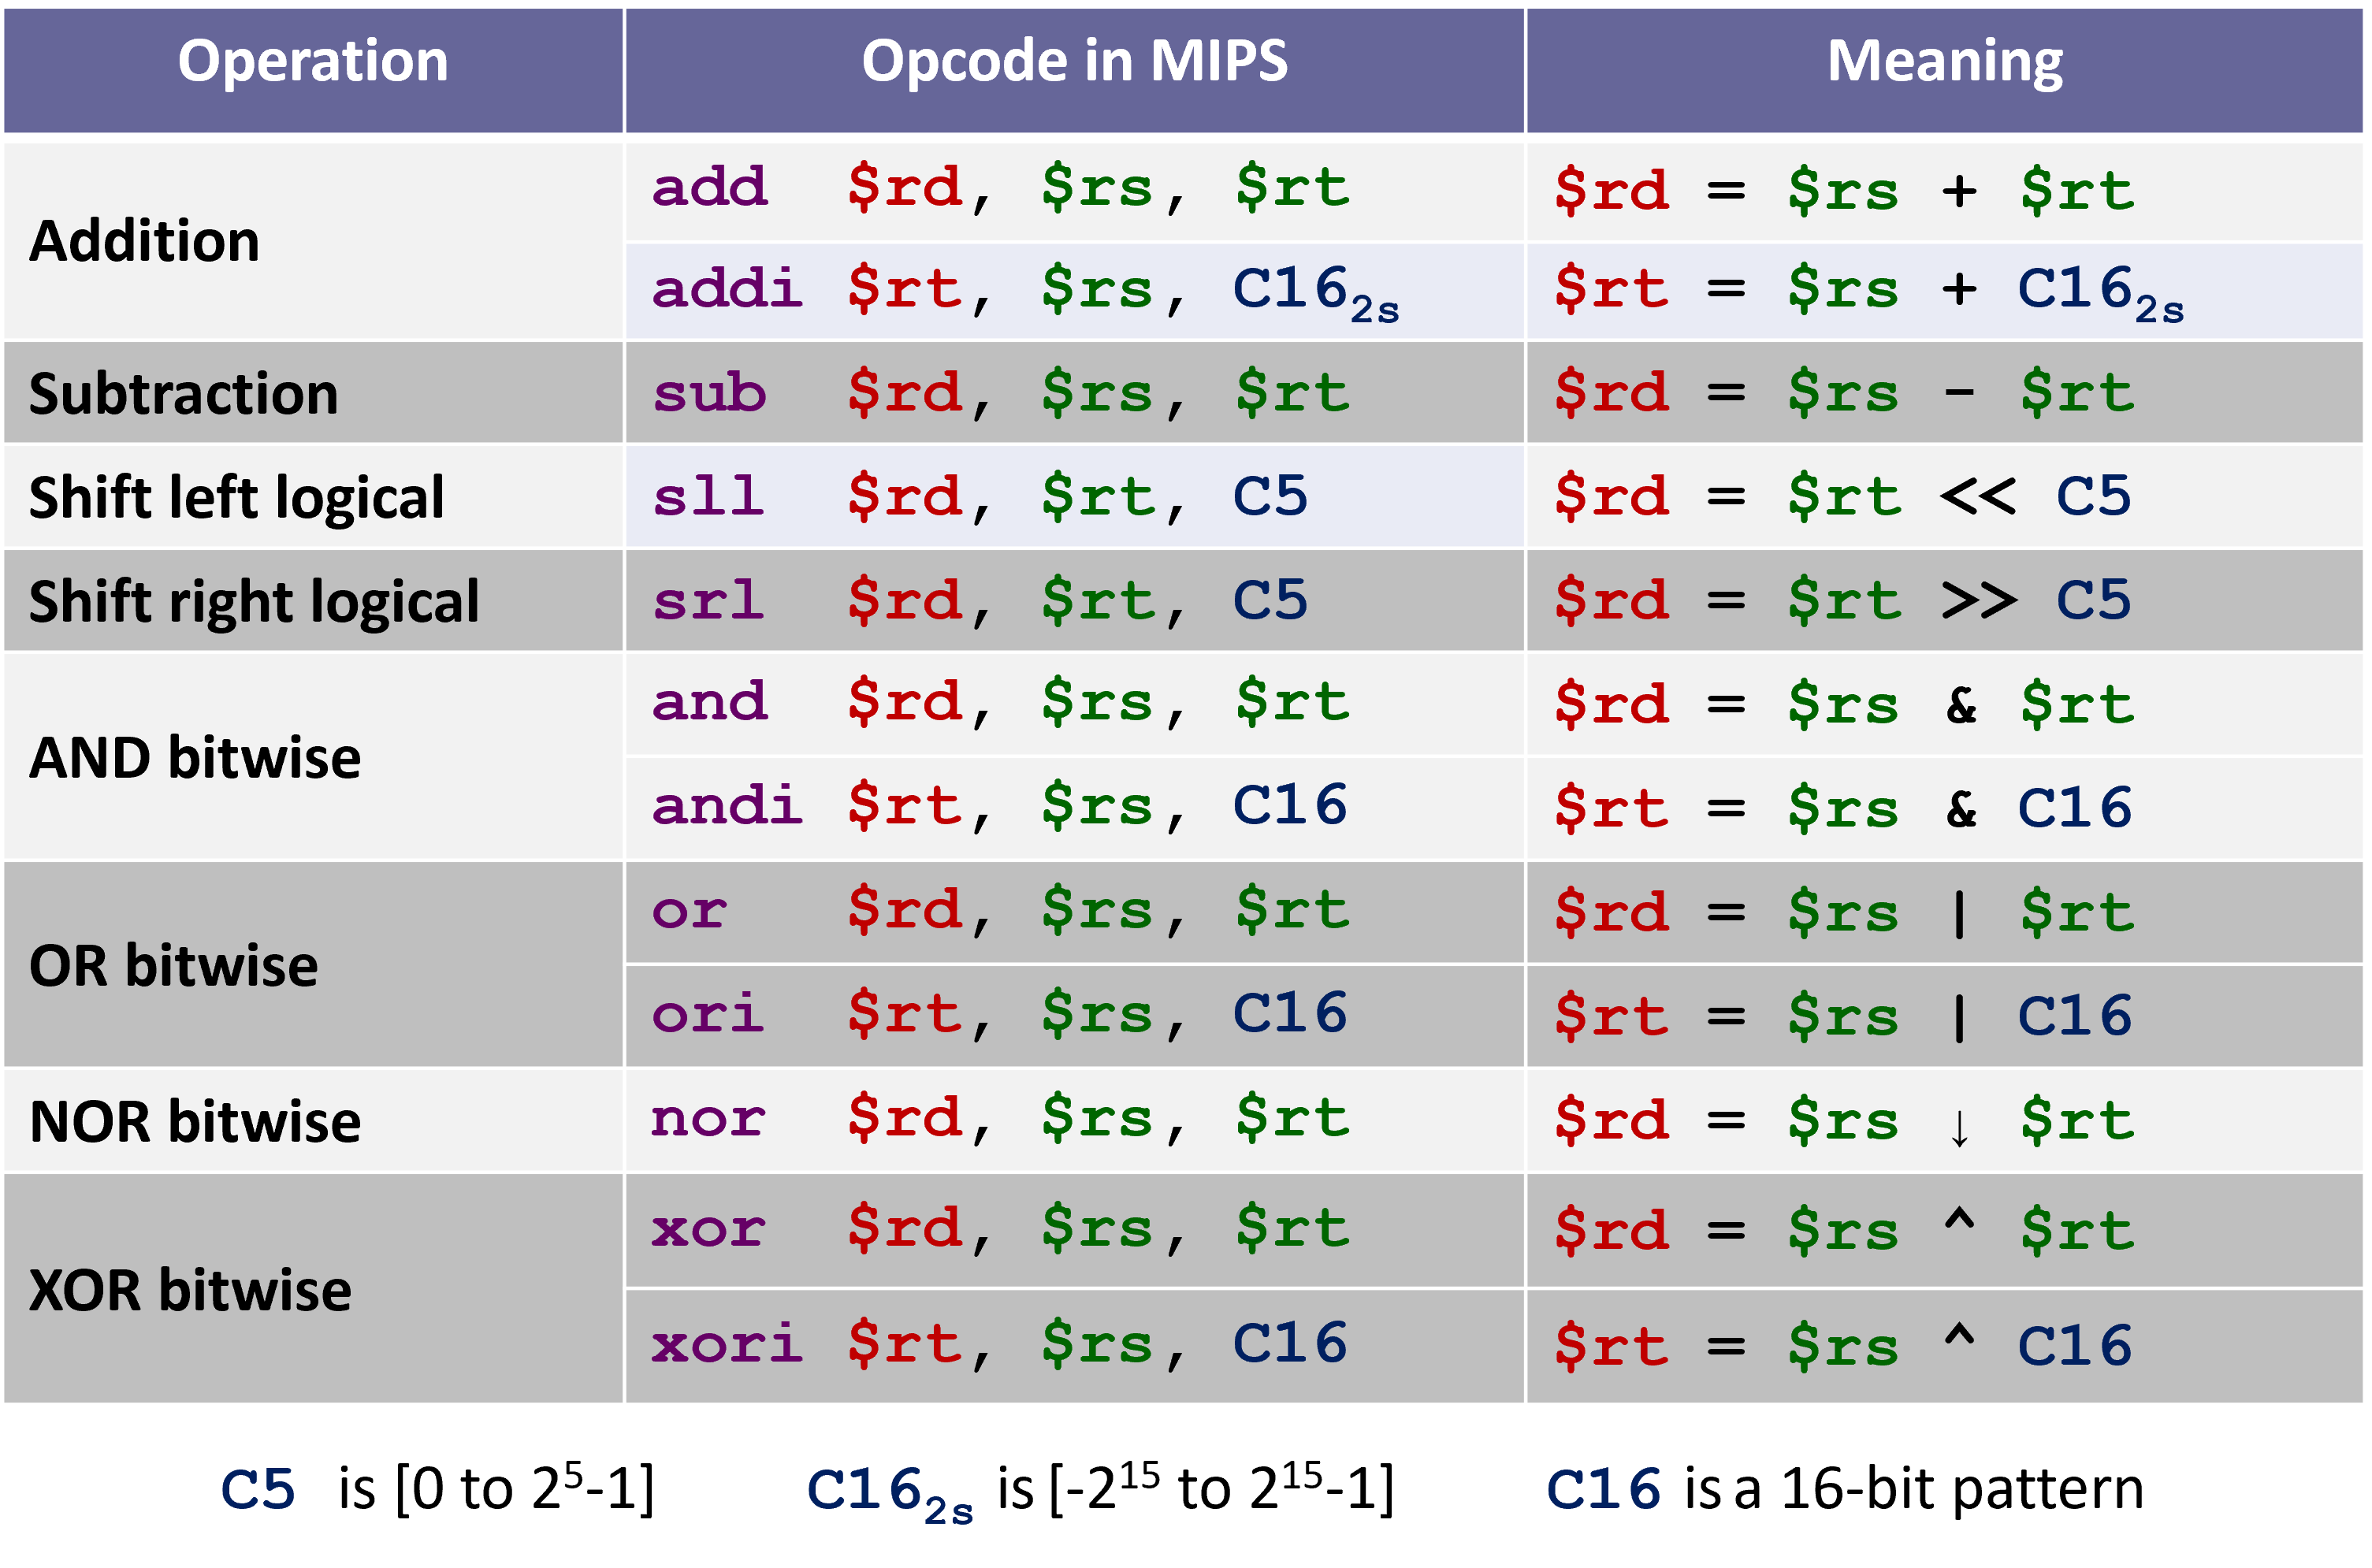
\includegraphics[width=0.8\linewidth]{mipsinstructions}}
\begin{itemize}
\item \code{add $s0, $s1, $zero} synonymous with \code{move $s0, $s1}
\item to get a \textbf{"NOT" operation}: \code{nor $t0, $t0, $zero}
 \item \code{lui} → load upper immediate (sets upper 16 bits of reg)
\end{itemize}

\textbf{Loading Large Constants}
\begin{itemize}
\item use \code{lui} to set the upper 16 bits (\code{lui $t0, 0xAAAA} ), lower bits filled with zeroes
\item use \code{ori} to set the lower-order bits (\code{ori $t0, $t0, 0xF0F0})
\end{itemize}

\textbf{Memory Instructions}
\begin{itemize}
\item \code{lw target, dis(src)}: load Mem[src+dis] content to target
\item \code{sw src, disp(target)}: store src content to Mem[targ+disp]
\item \code{lb / sb}: Load/Store byte (doesn't need word-align)
\end{itemize}

\textbf{Control Flow}
\begin{itemize}
\item \code{bne}: branch if Not Equal (\code{bne $t0, $t1, label})
\item \code{beq}: branch if Equal (\code{beq $t0, $t1, label} )
\item \code{j}: jump unconditionally (\code{beq $t0, $t1, label} )
\item \code{slt}: set to 1 on less than, else 0 (\code{slt dest, src1, src2} )
\end{itemize}

\subsubsection{MIPS Instructions Format}
\centerline{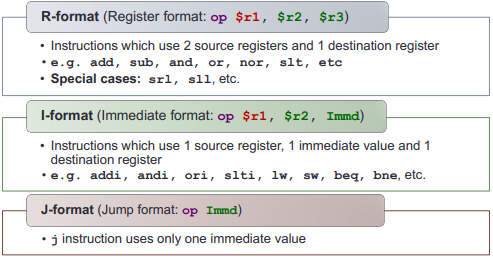
\includegraphics[width=0.9\linewidth]{instructionclass}}

\subsubsection{Memory Organisation}
\begin{itemize}
\item each location has an address: an index into the array \\
◦ for a k-bit address, the address space is of size $2^k$ \\
◦ largest address possible: $2^k - 1$, bc start from 0
\item byte addressing: one byte (8 bits) in every location/address \\
◦ more than one byte: word addressing
\item load-store architectures can only load data at \textbf{word boundaries} (divisible by n bytes) \\
e.g. If word consists of 4 bytes:
\end{itemize}
\centerline{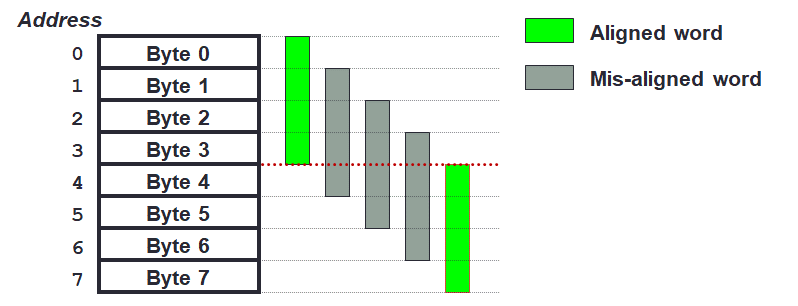
\includegraphics[width=0.9\linewidth]{wordalign}}

\subsubsection{MIPS:}
\begin{itemize}
\item Microprocessor without Interlocked Pipelined Stages
\item load-store register architecture \\
◦ 32 registers, each 32-bit (4 bytes) long \\
◦ each word contains 4 bytes \\
◦ memory addresses are 32-bit long
\item $2^{30}$ memory words ($2^{32}/4$) \\
◦ accessed only by data transfer instructions (aka \textbf{memory instructions})
\item MIPS uses byte addresses: consecutive words (word boundaries) differ by 4 \\
◦ e.g. Mem[0], Mem[4], ...
\end{itemize}


\vfill\null
\columnbreak



\section{7. MIPS Instruction Encoding}
Refer to \textbf{MIPS Reference Data} (midterms handout last slide)

\subsubsection{R Format:}
\centerline{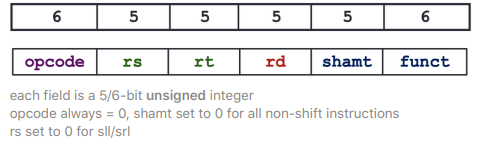
\includegraphics[width=0.9\linewidth]{Rformat}}

\subsubsection{I Format:}
\centerline{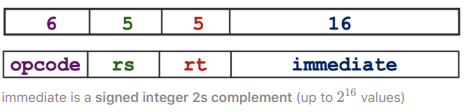
\includegraphics[width=0.9\linewidth]{Iformat}}

\subsubsection{J Format:}
\centerline{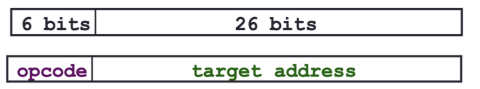
\includegraphics[width=0.9\linewidth]{Jformat}}
\begin{itemize}
\item  MIPS will take the 4 MSBs from PC+4 (next instruction after the jump
instruction)
\item omit 2 LSB (rightmost) since instruction addresses are word-aligned
\item maximum jump range = $2^{26+2+4} = 2^{32}$
\end{itemize}

\subsubsection{PC-Relative Addressing}
\begin{itemize}
\item Program Counter (PC): special register that keeps address of the
instruction being executed in the processor
\item target address = PC + 16-bit \code{immediate} field \\
◦ can branch $+- 2^{15}$ words = $2^{17}$ bytes from the PC \\
◦ interpret \code{immediate} as the number of words since instructions
are word-aligned: larger range!
\item next branch calculation: \\
◦ if branch is not taken: \textbf{PC+4} \\
◦ if branch is taken: \textbf{(PC+4) + (immediate x 4)}
\end{itemize}

\columnbreak

\subsubsection{Addressing Modes}
Addressing mode: ways to specify an operand in an assembly
\begin{itemize}
\item \textbf{Register Addressing}: operands are registers. (R format Instructions) \\
\centerline{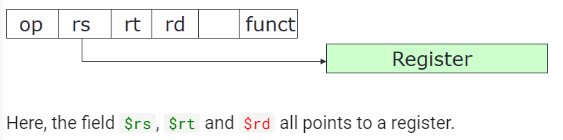
\includegraphics[width=0.9\linewidth]{registeraddressing}}

\item \textbf{Immediate Addressing}: operand is a constant within the instruction itself. e.g.\code{andi}, \code{addi}, \code{ori} \code{slti} etc. \\ \\
\centerline{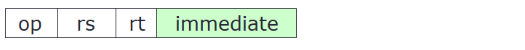
\includegraphics[width=0.9\linewidth]{immediateaddressing}}

\item \textbf{Base/Displacement Addressing}: operand is at the memory location whose address is the sum of a register and a constant in the instruction. 
\code{lw}, \code{sw}: (base address) + immediate (displacement) \\
\centerline{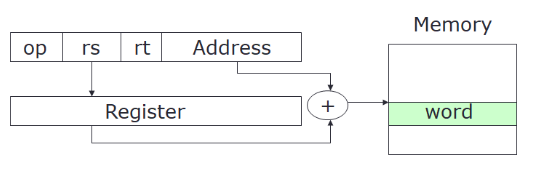
\includegraphics[width=0.9\linewidth]{baseaddressing}}

\item \textbf{PC-relative Addressing}: address is the sum of PC and constant in the instruction (e.g.\code{beq}, \code{bne}). \\ 
branch address is relative to PC+4 \\
\centerline{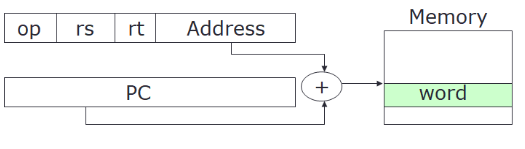
\includegraphics[width=0.9\linewidth]{pcrelativeaddressing}}

\item \textbf{Pseudo-direct Addressing}: 26-bit of instruction concatenated with the 4 MSBs of PC (e.g. \code{j} )
\centerline{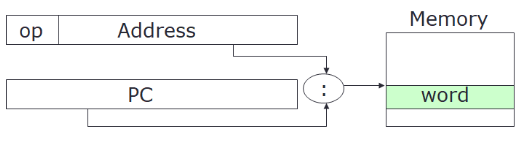
\includegraphics[width=0.9\linewidth]{pseudodirectaddressing}} \\
\centerline{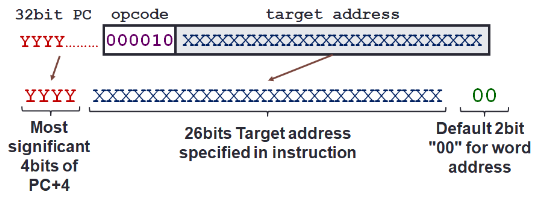
\includegraphics[width=0.7\linewidth]{pseudodirectaddressing2}}
\end{itemize}

\subsubsection{Summary}
\centerline{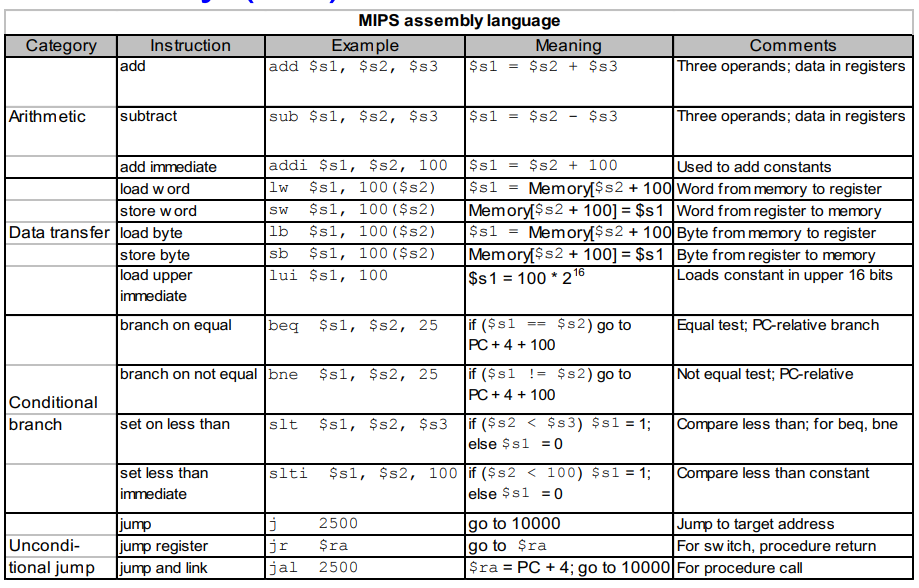
\includegraphics[width=1\linewidth]{MIPSsummary}}

\vfill\null
\columnbreak


\section{8. Instruction Set Architecture}
\subsubsection{1. Data Storage}
Concerned with where we store the operands so computation can be performed, store result afterwards, how to specify operands. \\
\textbf{Storage Architectures} \\
\centerline{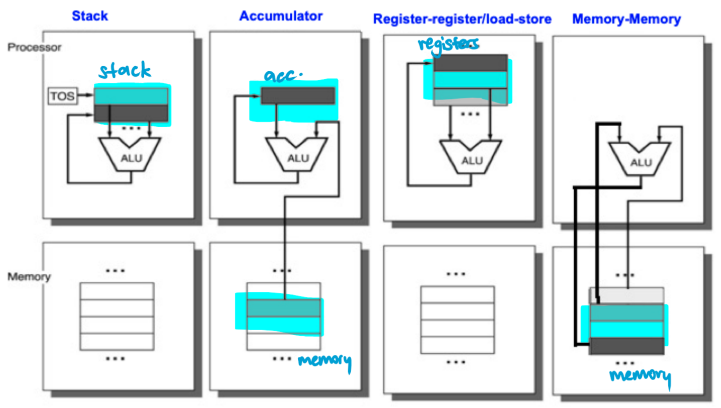
\includegraphics[width=1\linewidth]{storagearchitectures}}
\centerline{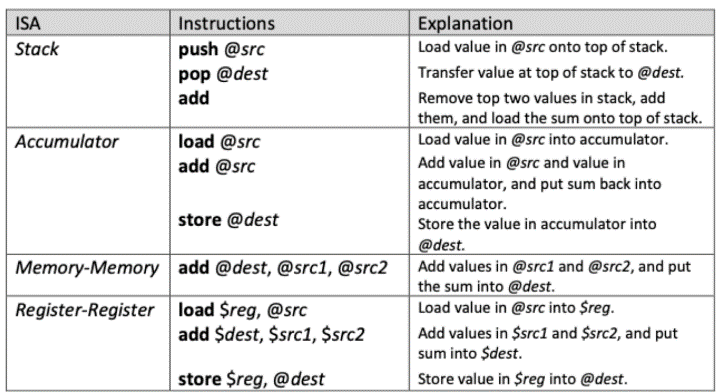
\includegraphics[width=1\linewidth]{ISAinstructions}}

\subsubsection{2. Memory Addressing Mode}
Concerned with memory locations and addresses, the addressing modes as well as the memory content.
\begin{itemize}
\item \textbf{endianness}: the relative ordering of bytes in a multiple-byte word stored in memory \\
◦ big endian: MSB stored in lowest address \\
◦ small endian → LSB stored in lowest address
\item \textbf{3 addressing modes in MIPS:} \\
1. register: operand is in a register (e.g. \code{add $t1, $t2, $t3}) \\
2. immediate: operand is specified directly in the instruction(e.g. \code{addi $t1, $t2, 98}) \\
3. displacement: operand is in memory with address calculated as base + offset (e.g. \code{lw $t1, 20($t2)}),
a form of immediate mode instruction
\end{itemize}


\subsubsection{3. Operations in the Instruction Set}
Every instruction set should have a set of standard operations \\
\centerline{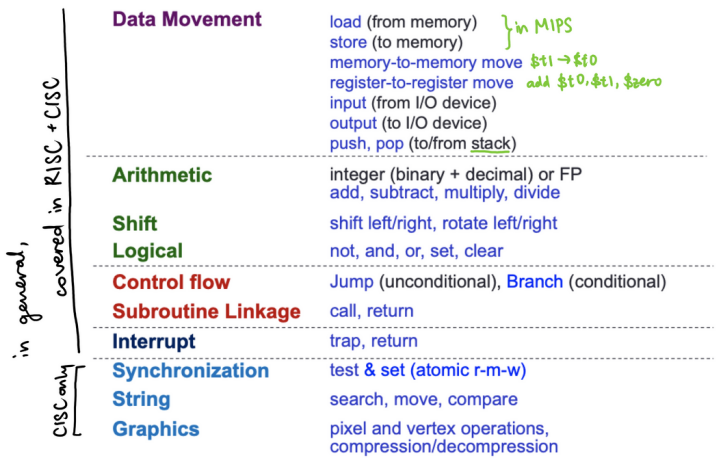
\includegraphics[width=1\linewidth]{ISoperations}}

\subsubsection{4. Instruction Formats}
Concerned with instruction length as well as instruction fields. In particular, for instruction fields, we are interested in the type and size of operands. \\ \\
\textbf{Instruction Length}:
\begin{itemize}
\item fixed-length instructions: \\
◦ easy fetch and decode \\
◦ simplified pipelining and parallelism \\
◦ instruction bits are scarce
\item variable-length instructions \\
◦ require multiple steps to fetch and decode instructions \\
◦ more flexible
\end{itemize}

\textbf{Instruction Fields}:
\begin{itemize}
\item type and size of operands (i.e. how to divide up the instructions)
\item instruction costs of: \\
◦ \textbf{opcode}: unique code to specify the desired operation:  \\
◦ designates the \textbf{type} and \textbf{size} of operands \\
◦ operands: zero or more additional information needed for the instruction
\item 32-bit architecture should support \\
◦ 8-, 16-, 32-bit integer operations \\
◦ 32- and 64-bit floating point operations
\end{itemize}

\subsubsection{5. Instruction Encoding}
\begin{itemize}
\item choice of variable/fixed/hybrid encoding
\item \textbf{expanding opcode scheme}: opcode variable lengths for different
instructions, maximise instruction bits\\
◦ use unused bits to define opcode, larger instruction set
\end{itemize}

\section{8.5 MIPS Processor}
• programmer writes program in high-level language (e.g. C) \\
•  \underline{compiler} translates to assembly language (MIPS) \\
•  \underline{assembler} translates to machine code (binaries) \\
•  \underline{processor} executes machine code (binaries) \\

\subsubsection{Building a Processor}
There are two major components of a processor:
\begin{itemize}
\item \textbf{Datapath}: \\
• Collection of components that process data. \\
• Performs the arithmetic, logical and memory operations. \\
• takes in data from operands, processes it, writes the data back.
\item \textbf{Control}: \\
• Tells the datapath, memory and I/O devices what to do according to program instructions. \\
• generates control signals.
\end{itemize}

\textbf{Goal}: Implement simplest possible implementation of a subset of the core MIPS ISA. \\
 In particular, we are interested only at the following operations:
\begin{itemize}
\item Arithmetic and Logical: \code{add}, \code{sub}, \code{and}, \code{or}, \code{slt}, \code{andi1}*, \code{ori1}* \\
(* Not fully implementable in simplest implementation, as we do "sign extension" on immd value).
\item Data Transfer: \code{lw} and \code{sw}
\item Branches: \code{beq} and \code{bne}
\end{itemize}

\vfill\null
\columnbreak

\section{9. Datapath}
\subsubsection{Instruction Execution Cycle}
\centerline{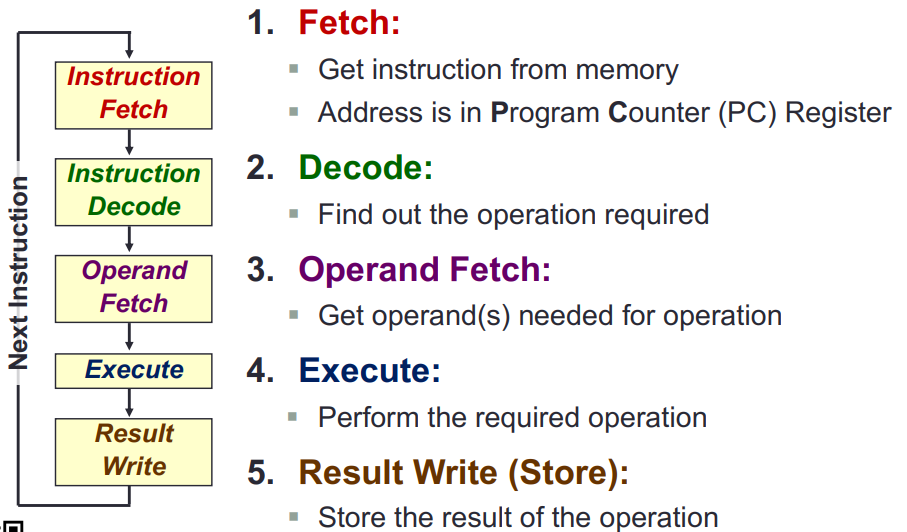
\includegraphics[width=0.8\linewidth]{IEC}}

\subsubsection{in MIPS}
\centerline{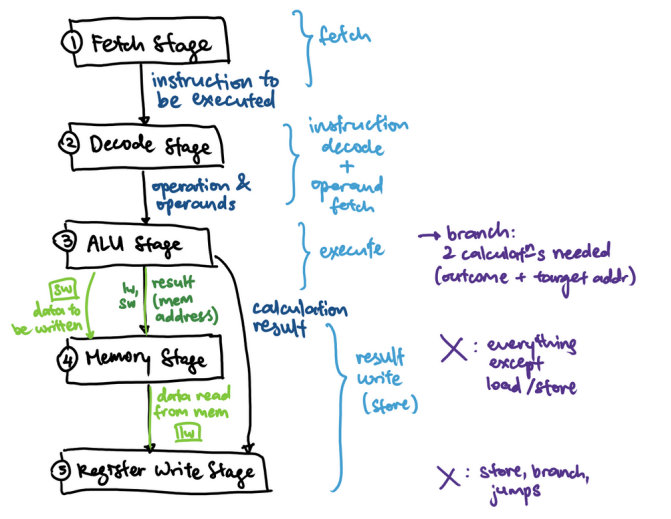
\includegraphics[width=0.8\linewidth]{IECMIPS}}

\subsubsection{1. Fetch Stage}
Fetch instruction and prepares the processor to get the next instruction.
\begin{itemize}
\item use PC to fetch instruction from memory
\item increment PC by 4 to get the next instruction (using an Adder)
\item output (to Decode): instruction to be executed
\end{itemize}

\subsubsection{2. Decode Stage}
Decode stage is combined with the operand fetch stage due to the simplicity of the pure decode stage.
\begin{itemize}
\item gathers data from the instruction fields \\
1. read opcode and determine the instruction type and field lengths \\
2. read data from all necessary registers
\item output (to ALU): operation and the necessary operands
\end{itemize}

\subsubsection{3. ALU (execution) Stage}
\begin{itemize}
\item output (to memory stage): calculation result
\end{itemize}

\subsubsection{4. Memory Stage}
\begin{itemize}
\item only \code{load}, \code{store} instructions needed to perform operations in this stage \\
◦ uses memory address calculated by ALU stage (input)
\item all other instructions are idle in this stage \\
◦ result from ALU stage will pass through this stage to be used in Register Write stage
\item inputs: \\
◦ computation result to be used as memory address \\
◦ register value to be written to memory (only \code{sw})
\item outputs (to Register Write stage): result to be stored (only \code{lw})
\end{itemize}

\subsubsection{5. Register Write Stage}
\begin{itemize}
\item write the result of some computation into a register \\
◦ do nothing: stores / branches / jumps
\item input: \\
◦ destination register number \\
◦ computation result (from either memory or ALU)
\end{itemize}

\section{9.5 Datapath Elements}
\subsubsection{Instruction Memory [1, Fetch]}
\begin{itemize}
\item Storage element for the instructions (Sequential circuit).
\item supplies instructions given an address \\
◦ input: instruction address M \\
◦ outputs: contents of address M (binary pattern of instructions)
\end{itemize}

\subsubsection{Adder [1]}
\begin{itemize}
\item combinational logic to add two numbers. \\
\centerline{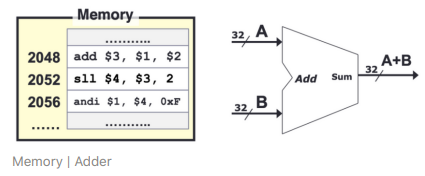
\includegraphics[width=0.6\linewidth]{adder}}
\end{itemize}

\subsubsection{Clock [1]}
\begin{itemize}
\item a square wave used by the processor \\
◦ times operations inside the processor (e.g. reading \& updating PC)
\item allows read and update of PC at the same time \\
◦ PC is read during the first half of the clock period \\
◦ PC is updated only at the rising edge \\ \\
\centerline{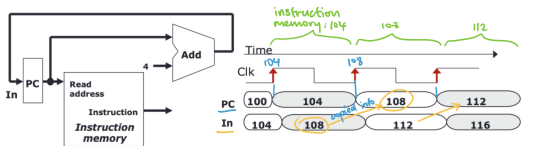
\includegraphics[width=0.9\linewidth]{clock}}
\end{itemize}

\subsubsection{Register File [2]}
\begin{itemize}
\item collection of 32 registers (each 32 bits wide) \\
◦ can be read by specifying register number
\item read at most 2 registers per instruction 
\item write at most one register per instruction
\item \code{RegWrite}: control signal to indicate writing of register \\
\end{itemize}
\centerline{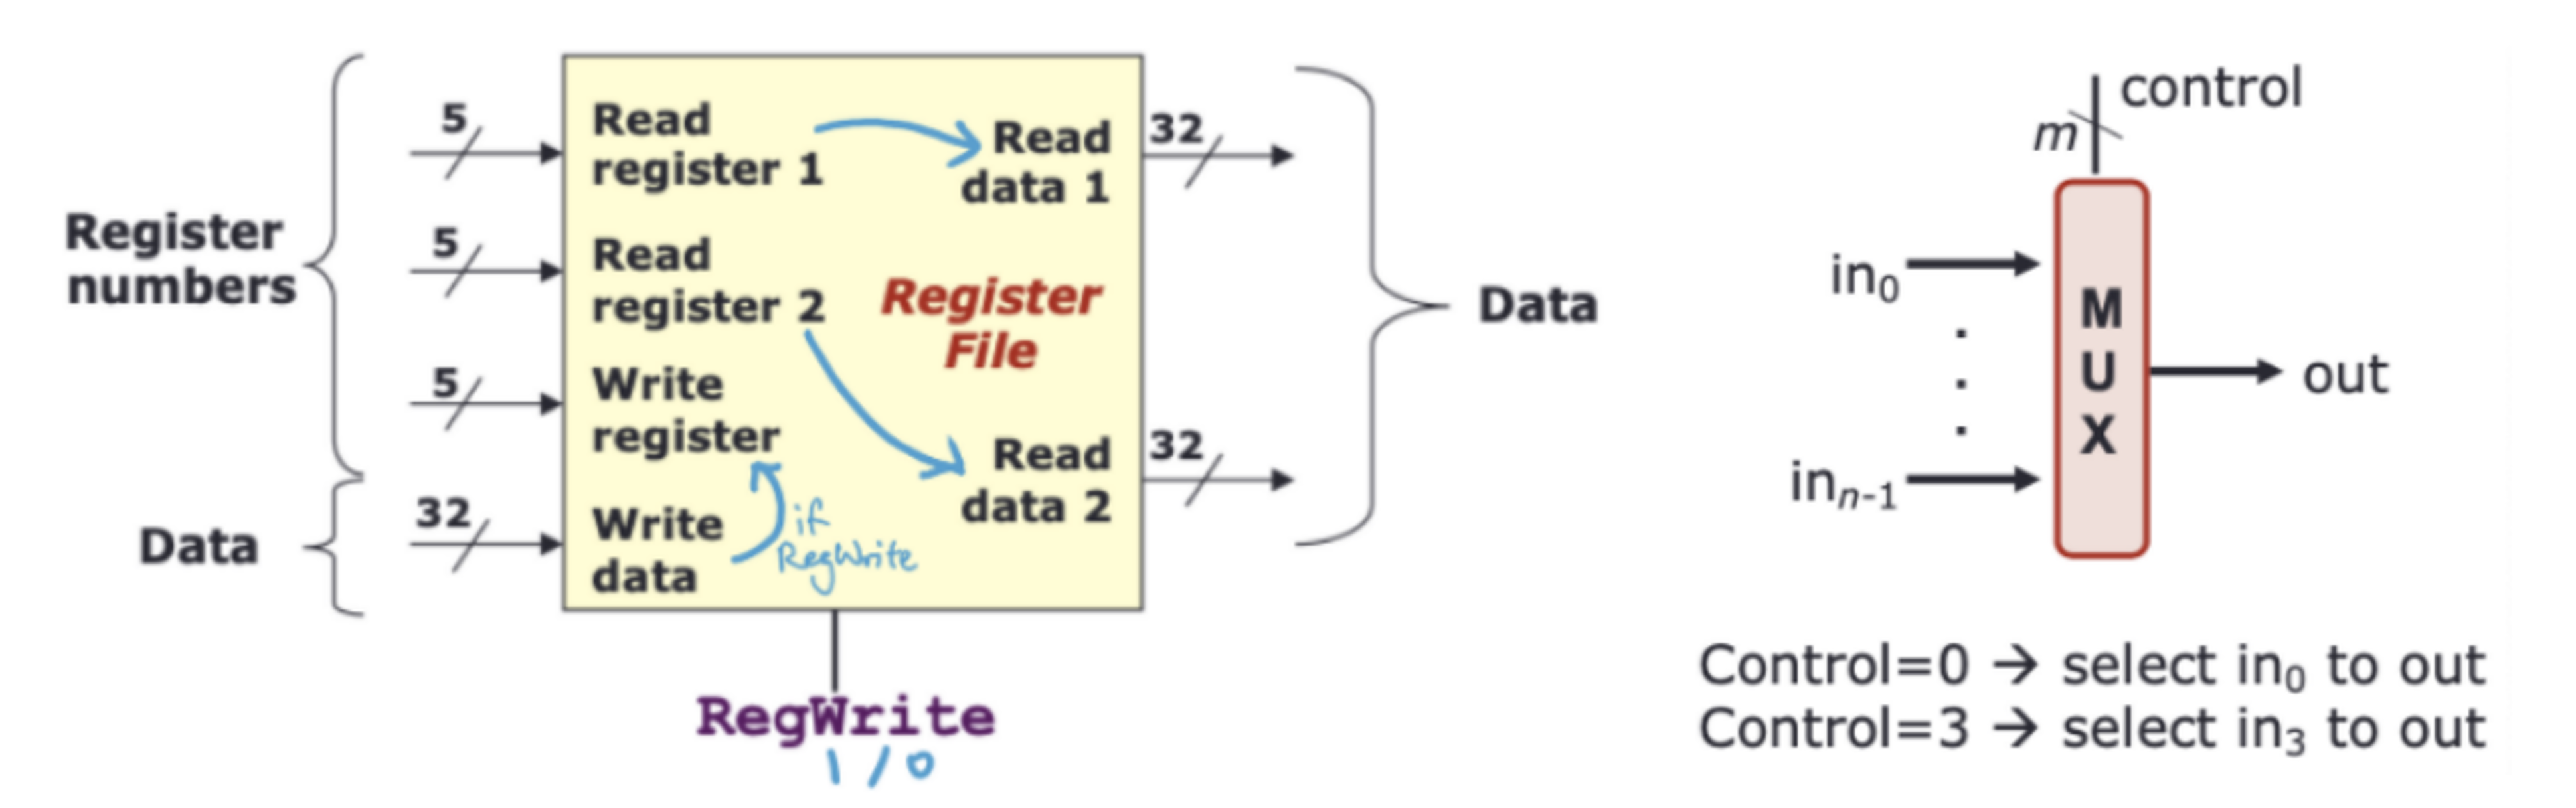
\includegraphics[width=0.9\linewidth]{regfilemulti}}

\subsubsection{Multiplexer}
\begin{itemize}
\item  selects one input from multiple input lines \\
◦ inputs: $n$ lines of same width \\
◦ outputs: select input $i^{th}$ line if control = $i$ \\
◦ control: $m$ bits where $n$ = $2^m$
\end{itemize}

\vfill \null
\columnbreak

\subsubsection{ALU [3]}
\begin{itemize}
\item combinational logic to implement arithmetic and logical operations
\item inputs: two 32-bit numbers
\item outputs: \\
◦ result of arithmetic/logical operation \\
◦ 1-bit signal to indicate whether result is zero
\item control (\code{ALUcontrol}): 4-bit to decide the operation \\
◦ set using opcode + funct field
\item 2 calculations needed for branch instructions (branch outcome +
branch target address)
\end{itemize}

\centerline{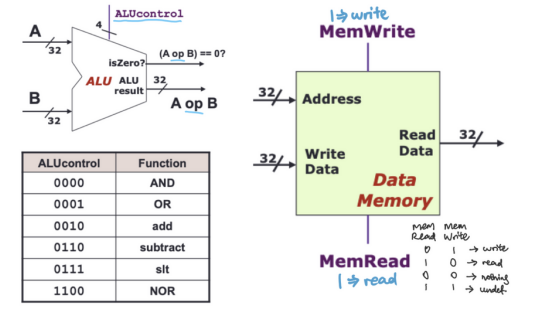
\includegraphics[width=0.9\linewidth]{alumem}}

\subsubsection{Data Memory [4]}
\begin{itemize}
\item storage element for the data of a program
\item inputs: memory address \\
◦ data to be written (for store instructions)
\item outputs: data read from memory (for load instructions)
\item control: \code{MemRead} and \code{MemWrite} controls \\
◦ only one can be asserted at any point in time
\end{itemize}


\section{10. Control}
\subsubsection{Control Signals}
These can be generated using opcode directly.
\begin{itemize} 

\item \code{RegDst} @ Decode/Operand Fetch \\
◦ 0/1: write register = \code{Inst[20:16]} / \code{Inst[15:11]}
\item \code{RegWrite} @ Decode/Operand Fetch \\
◦ 0/1: No register write / WD written to WR
\item \code{ALUSrc} @ ALU (determines first input) \\
◦ 0: \code{Operand2 = Register Read Data 2} \\
◦ 1: \code{Operand2 = SignExt(Inst[15:0])} (sign ext immediate)
\item \code{MemRead} @ Memory \\
◦ 0/1: no read / reads memory using Address (returned in RD)
\item \code{MemWrite} @ Memory \\
◦ 0/1: no write / writes Register RD 2 into mem[Address]
\item \code{MemToReg} @ RegWrite \\
◦ 0/1 → register write data = ALU result / memory read data
\item \code{PCSrc @ Memory/RegWrite} \\
◦ 0/1 → next PC = PC + 4 / PC = SignExt(Inst[15:0]) << 2 + (PC + 4) \\
◦ PCSrc = set to 1 if Branch AND is0 are both 1 \\
◦ aka (isBranchInstruction AND branchIsTaken)
\end{itemize}
\centerline{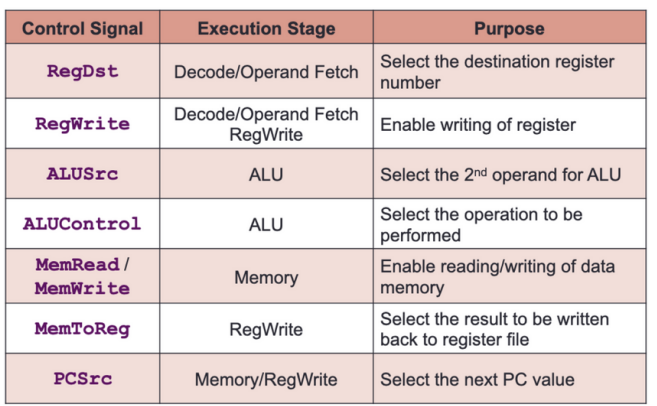
\includegraphics[width=0.9\linewidth]{signals1}}

\subsubsection{ALU}
\centerline{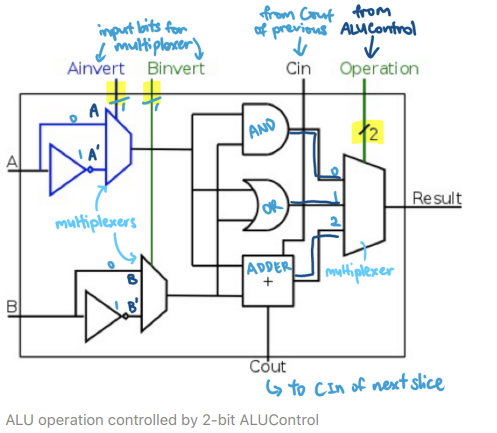
\includegraphics[width=0.7\linewidth]{ALU}}

\subsubsection{Controller Design}
Determines Control Signals from Opcode \\
\centerline{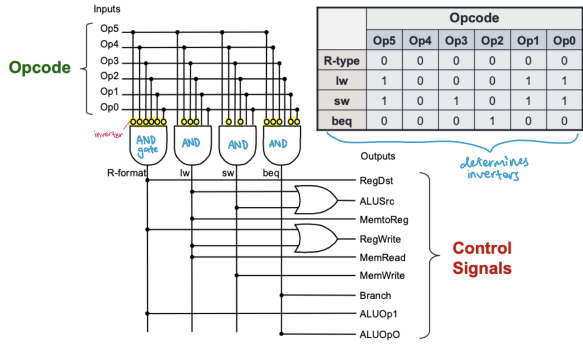
\includegraphics[width=0.8\linewidth]{controllerdesign}}

\subsubsection{Multilevel Decoding}
\begin{itemize}
\item to determine ALUControl signal \\
◦ depends on 12 variables (6-bit opcode + 6-bit funct)
\item reduce the number of cases, then generate the full output \\
◦ reduce the size of the main controller - simplify design process
\item how it works \\
1. use opcode to generate 2-bit \code{ALUop} signal \\
2. use \code{ALUop} signal and funct (for R-type) to generate 4-bit \code{ALUcontrol} sign
\end{itemize}
\centerline{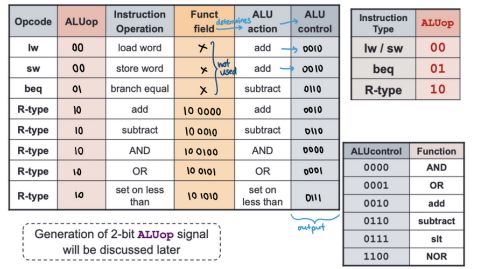
\includegraphics[width=0.8\linewidth]{multilevel1}} 
\centerline{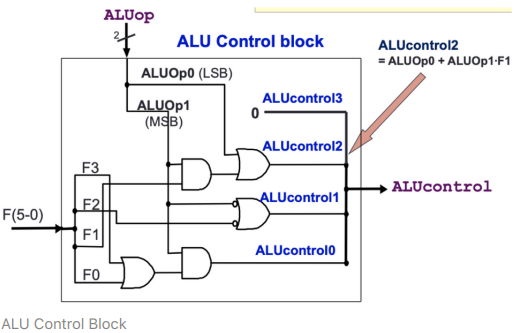
\includegraphics[width=0.8\linewidth]{multilevel2}}

% Diagrams: AND CONTROL FLOW DETERMINATION
\end{multicols*}
\begin{multicols*}{2}
\subsubsection{Complete Datapath}
\centerline{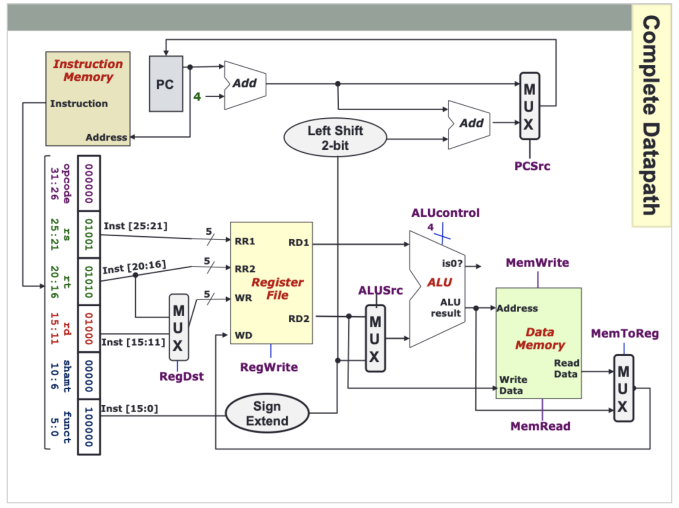
\includegraphics[width=1\linewidth]{completedatapath}}
\bigskip
\subsubsection{ALUcontrol on ALU}
\centerline{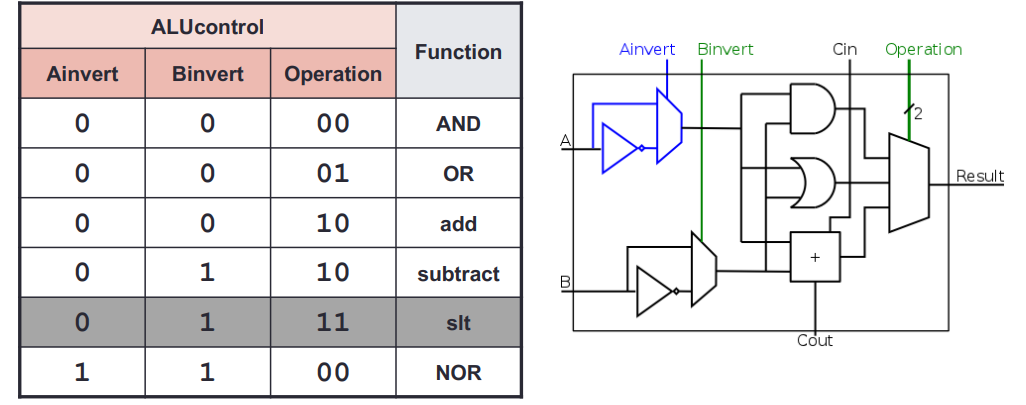
\includegraphics[width=1\linewidth]{ALUcontrolonALU}}


\vfill \null
\columnbreak
\subsubsection{Complete Datapath and Control}
\centerline{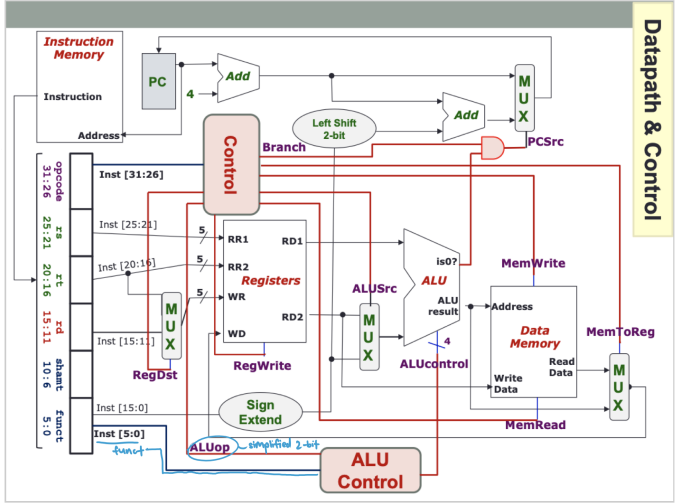
\includegraphics[width=1\linewidth]{datapathandcontrol}}
\bigskip
\subsubsection{Control Design: Outputs}
\centerline{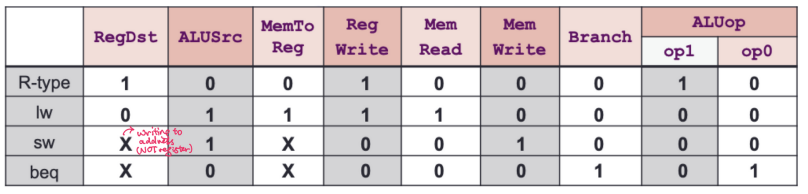
\includegraphics[width=1\linewidth]{controldesignoutputs}}
\end{multicols*}
\begin{multicols*}{2}
\section{Control Flow Determination}
\subsubsection{Control Signals}
\begin{itemize} 
\item \code{RegDst} @ Decode/Operand Fetch \\
◦ 0/1: write register = \code{Inst[20:16]} / \code{Inst[15:11]}
\item \code{RegWrite} @ Decode/Operand Fetch \\
◦ 0/1: No register write / WD written to WR
\item \code{ALUSrc} @ ALU (determines first input) \\
◦ 0: \code{Operand2 = Register Read Data 2} \\
◦ 1: \code{Operand2 = SignExt(Inst[15:0])} (sign ext immediate)
\item \code{MemRead} @ Memory \\
◦ 0/1: no read / reads memory using Address (returned in RD)
\item \code{MemWrite} @ Memory \\
◦ 0/1: no write / writes Register RD 2 into mem[Address]
\item \code{MemToReg} @ RegWrite \\
◦ 0/1 → register write data = ALU result / memory read data
\item \code{PCSrc @ Memory/RegWrite} \\
◦ 0/1 → next PC = PC + 4 / PC = SignExt(Inst[15:0]) $<<$ 2 + (PC + 4) \\
◦ PCSrc = set to 1 if Branch AND is0 are both 1 \\
◦ aka (isBranchInstruction AND branchIsTaken)
\end{itemize}

\subsubsection{Control Design: Outputs}
\centerline{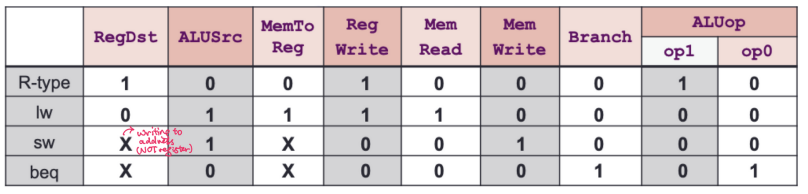
\includegraphics[width=0.8\linewidth]{controldesignoutputs}}
\centerline{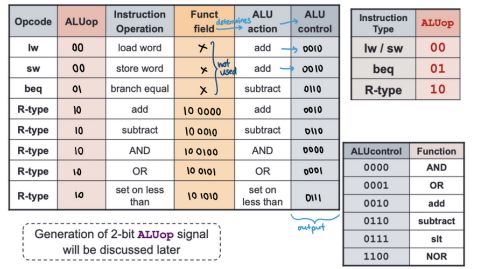
\includegraphics[width=0.8\linewidth]{multilevel1}} 
\subsubsection{Complete Datapath}
\centerline{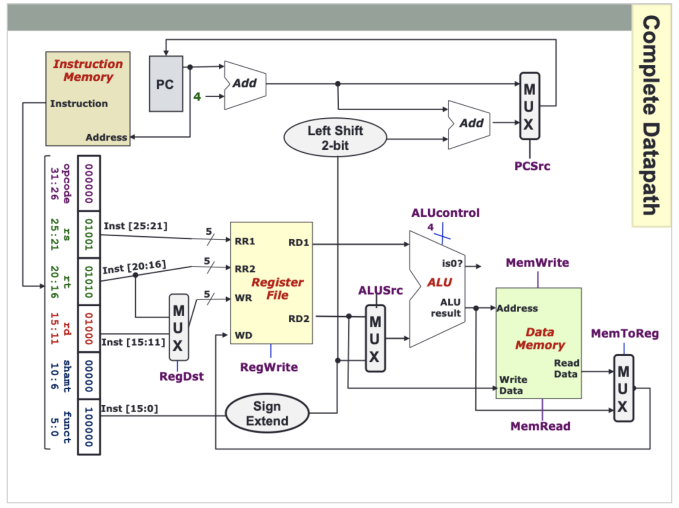
\includegraphics[width=0.9\linewidth]{completedatapath}}
\subsubsection{Complete Datapath and Control}
\centerline{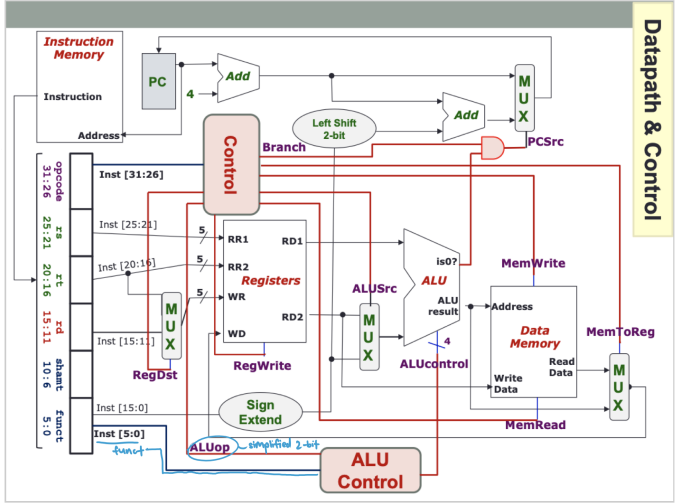
\includegraphics[width=0.9\linewidth]{datapathandcontrol}}

\end{multicols*}
\begin{multicols*}{3}

\section{11. Instruction Execution}
\subsubsection{Instruction Execution}
\begin{itemize}
\item coordinating the stages together: fetch, decode, memory, write etc
\end{itemize}

\subsubsection{Single Cycle Implementation}
\begin{itemize}
\item  how it works \\
1. read contents of one or more storage elements \\
2. perform computation through some combinational logic \\
3. write results to one or more storage elements (register/memory)
\item All performed \textbf{within a clock period} \\
◦ avoids reading a storage element when it's being written
\centerline{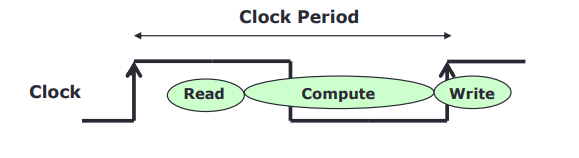
\includegraphics[width=0.8\linewidth]{singlecycle}}
\item time taken depends on slowest instruction
\item \textbf{disadvantage}: \\
◦ clock cycle must be long enough to accommodate the slowest instruction: all instructions will take the same time as the slowest
instruction.
\end{itemize}

\subsubsection{Multicycle Implementation}
\begin{itemize}
\item how it works: break up the instruction into execution steps \\
1. instruction fetch \\
2. instruction decode and register read \\
3. ALU operation\\
4. memory read/write\\
5. register write\\
◦ each execution step takes one clock cycle
\item time taken depends on number of steps \\
◦ cycle time is determined by the slowest step
\item disadvantage \\
◦ may not necessarily be faster - depends on mix of instructions
\end{itemize}

\subsubsection{Critical Path}
\begin{itemize}
\item \textbf{Critical Path}: The Critical Path is longest path from start to finish, indicating minimum time necessary to complete the entire operation.
\item Path critical as any delay along path delays completion of operation. Critical path is bottleneck route.
\item Applications in project management, resource allocation, scheduling, etc.
\end{itemize}

\subsubsection{Cycle Time (Propagation Delay)}
\begin{itemize}
\item For a \textbf{single cycle implementation}, (given component resource latencies), consider propagation delay of  instruction processing as critical (longest) path. 
\item Sum up latencies of critical path and disregard faster parallel paths.
\item \textbf{SUB (R-type) Critical path}: I-Mem $>$ Reg.File $>$ MUX(ALUSrc)  $>$ ALU  $>$ MUX(MemToReg)  $>$ Reg.File
\item \textbf{LW Critical Path}: I-Mem  $>$ Reg.File  $>$ ALU  $>$ DataMem  $>$ MUX(MemToReg)  $>$ Reg.File
\end{itemize}
\subsubsection{E.g. Critical Path for LW load word Instruction}
\centerline{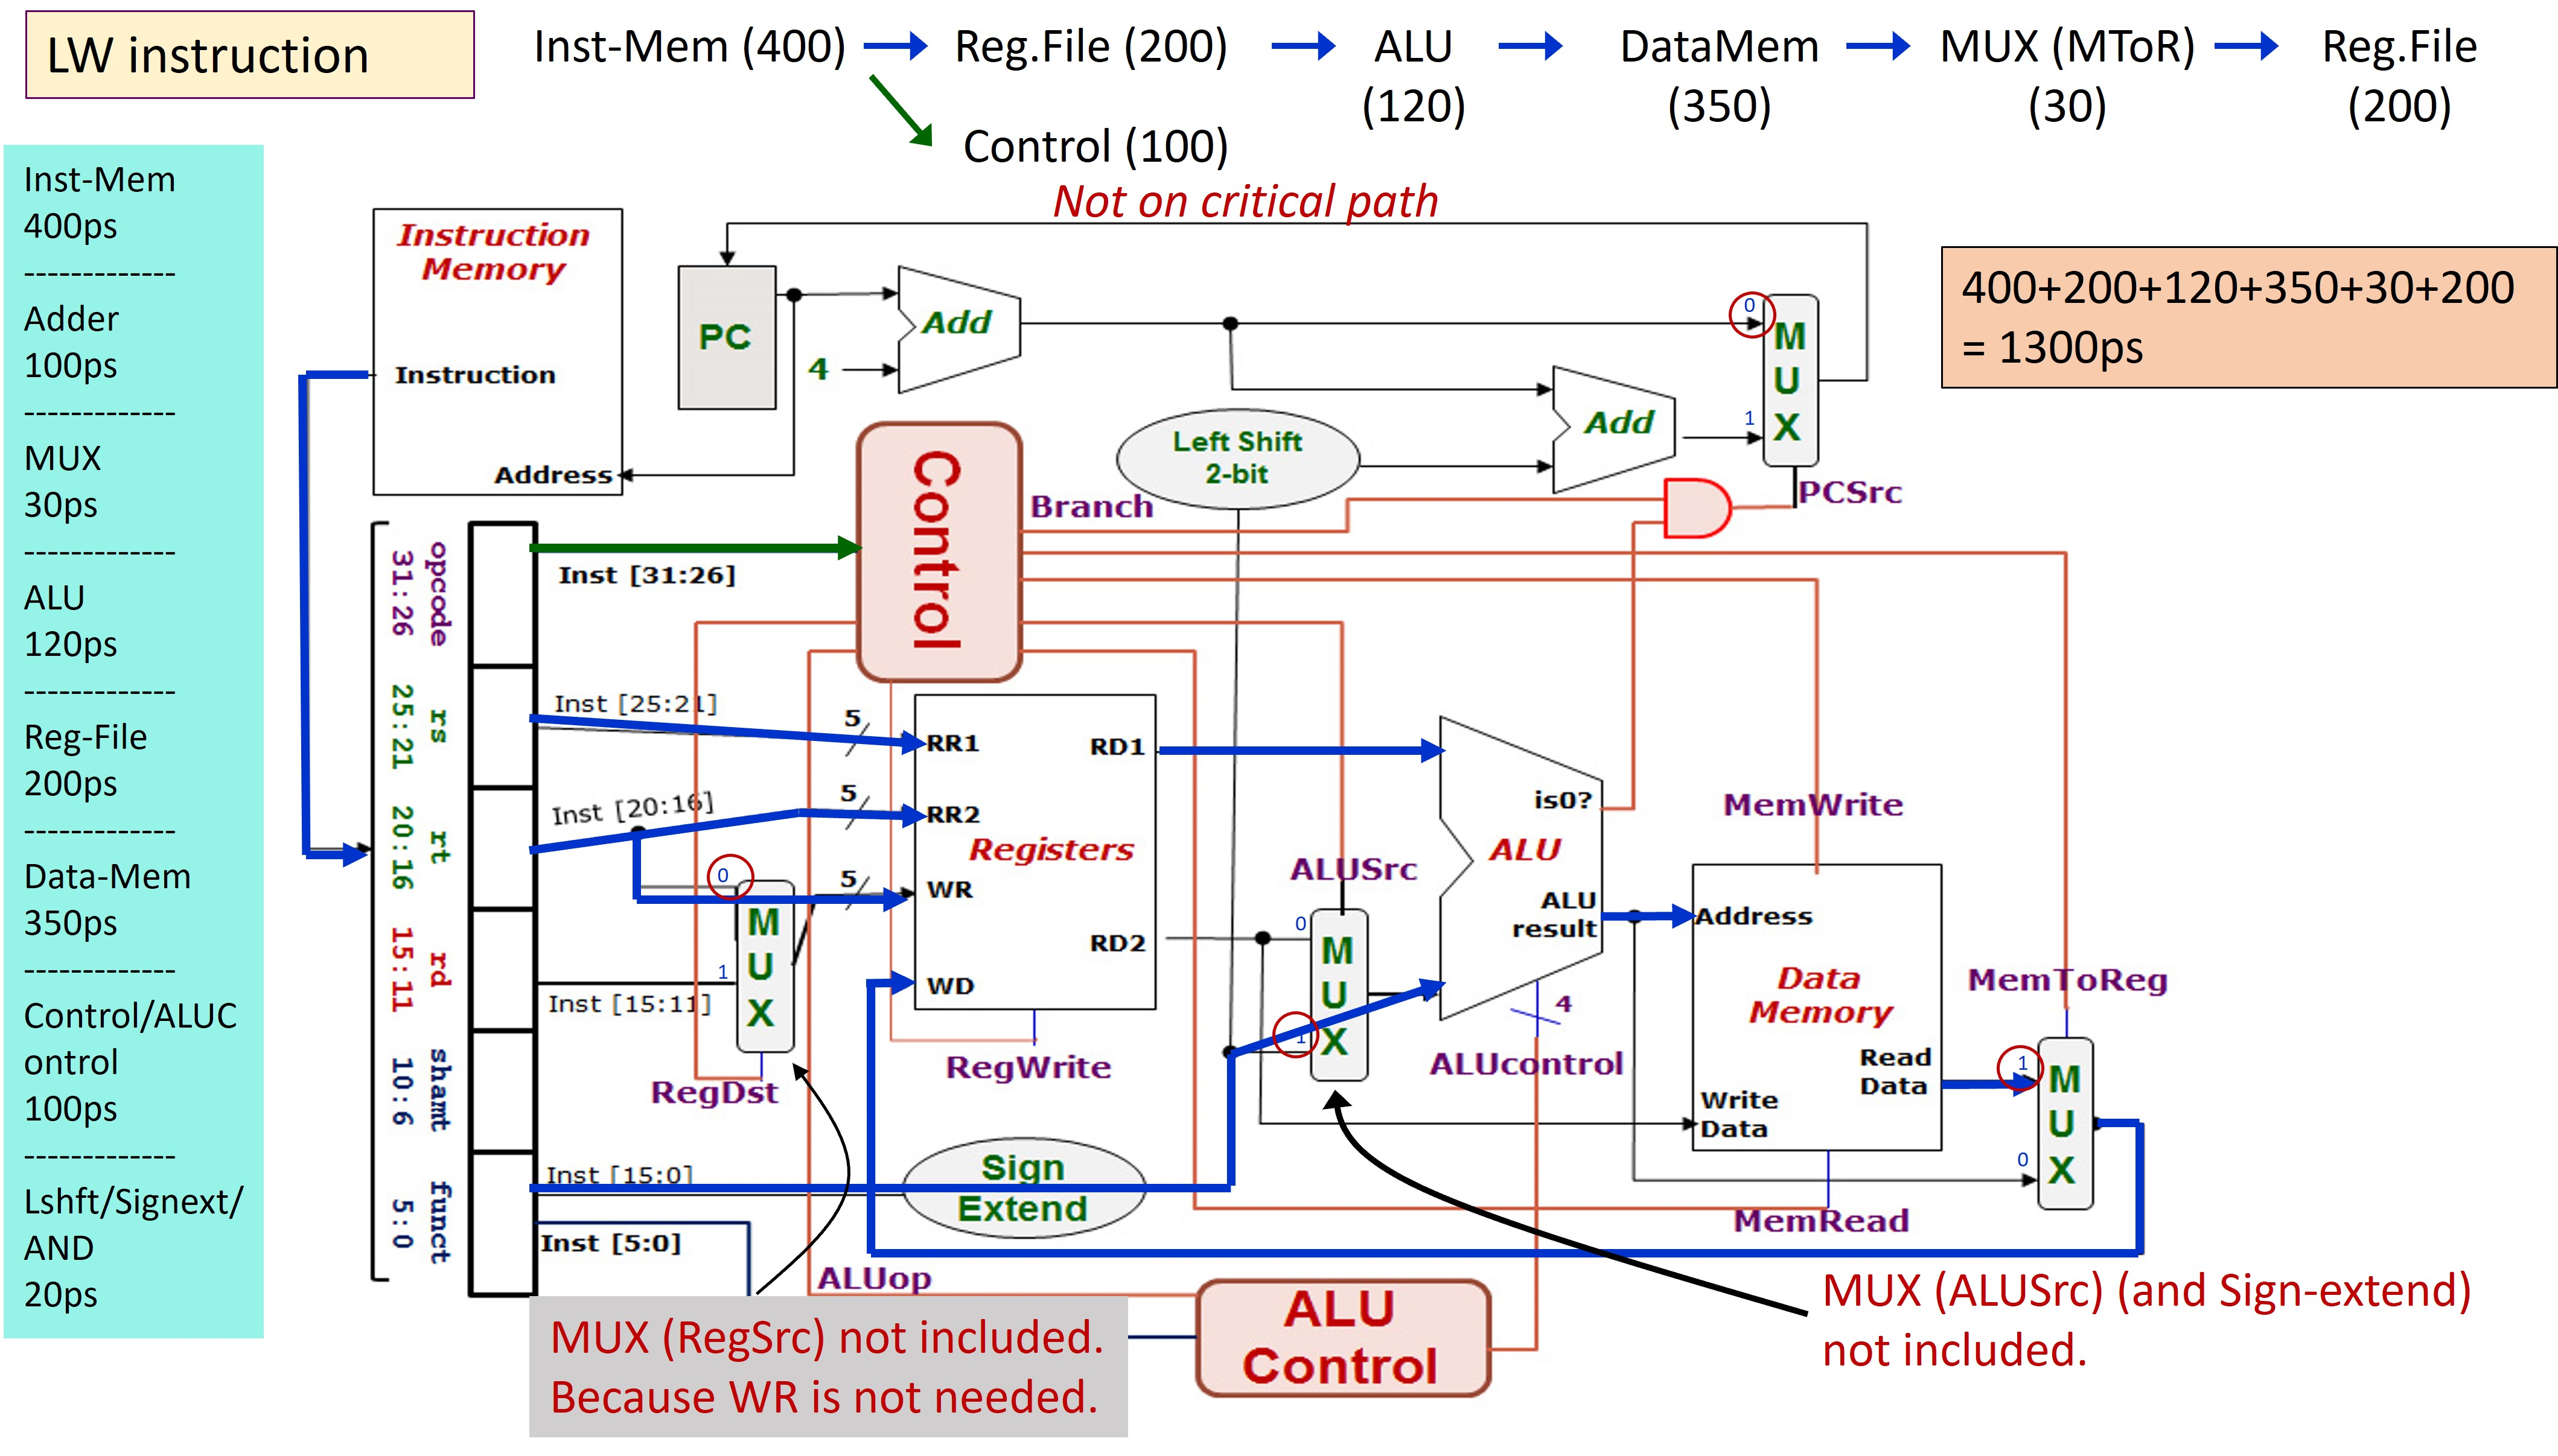
\includegraphics[width=1\linewidth]{LWcriticalpath}}

\subsubsection{Pipelining}
\begin{itemize}
\item Break up the instructions into execution steps 
one per clock cycle
\item Allow different instructions to be in different 
execution steps simultaneously
\end{itemize}














  
\end{multicols*}
\end{document}